\pdfminorversion=7
\documentclass[aspectratio=169,11pt]{beamer}

\IfFileExists{beamerthemeCCM.sty}{%
  \usetheme{CCM}
}{%
  \usetheme{default}
  \definecolor{CCMorange}{HTML}{F6862D}
  \definecolor{SFdark}{HTML}{1D2954}
  \definecolor{mygray}{HTML}{8F8F8F}
  \setbeamertemplate{navigation symbols}{}
  \setbeamertemplate{footline}[frame number]
  \setbeamersize{text margin left=0.25in,text margin right=0.25in}
  \setbeamercolor{title}{fg=CCMorange}
  \setbeamercolor{frametitle}{fg=CCMorange,bg=white}
  \setbeamercolor{item}{fg=CCMorange}
  \setbeamercolor{block title}{fg=black,bg=CCMorange!30}
  \setbeamercolor{block body}{fg=black,bg=black!3}
}

\usepackage{amsmath,amssymb,mathtools,mathrsfs}
\usepackage{bm}
\usepackage{booktabs}
\usepackage{graphicx}
\usepackage{times}
\usepackage{tikz}
\usepackage{pgfplots}
\usepackage{relsize}
\usetikzlibrary{arrows.meta,calc,positioning,decorations.pathreplacing,spy}
\pgfplotsset{compat=1.18}

\graphicspath{{day4_afternoon_figures/}}

\newcommand{\R}{\mathbb{R}}
\newcommand{\C}{\mathbb{C}}
\newcommand{\cO}{\mathcal{O}}
\newcommand{\dd}{\,\mathrm d}
\newcommand{\ii}{\mathrm i}
\newcommand{\x}{\bm{x}}
\newcommand{\xp}{\bm{x}'}
\newcommand{\kvec}{\bm{k}}
\newcommand{\rvec}{\bm{r}}
\newcommand{\rp}{\bm{r}'}
\newcommand{\nuvec}{\bm{\nu}}
\newcommand{\tvec}{\bm{t}}
% Shared operator notation for the AMSS FIEM talk slides.
% Change this one line to change the font for layer and volume potentials.
\newcommand{\FIEMopfont}[1]{\mathcal{#1}}

\newcommand{\Sop}{\FIEMopfont{S}}
\newcommand{\Dop}{\FIEMopfont{D}}
\newcommand{\Spop}{\Sop^{\prime}}
\newcommand{\Dpop}{\Dop^{\prime}}
\newcommand{\Vop}{\FIEMopfont{V}}
\newcommand{\Iop}{\FIEMopfont{I}}
\newcommand{\Kop}{\FIEMopfont{K}}
\newcommand{\KopT}{\Kop^{\prime}}
\newcommand{\Wop}{\FIEMopfont{W}}
\newcommand{\Aop}{\FIEMopfont{A}}
\newcommand{\Top}{\FIEMopfont{T}}

\newcommand{\hl}[1]{{\color{CCMorange}\textbf{#1}}}
\DeclareMathOperator{\erf}{erf}
\DeclareMathOperator{\erfc}{erfc}
\DeclareMathOperator{\rect}{rect}
\DeclareMathOperator{\sgn}{sgn}
\DeclareMathOperator{\Span}{span}

\title{Day 4 Afternoon: Poisson-NUFFT and RRQ}
\subtitle{Heat-potential nonuniform FFTs and recursive reduction quadrature}
\author{Fast Algorithms and Integral Equation Methods}
\institute{AMSS Summer Course}
\date{July 2026}

\setlength{\emergencystretch}{3em}

\begin{document}

% 1
\begin{frame}
  \titlepage
\end{frame}

% 2
\begin{frame}{Afternoon roadmap}
\footnotesize
\begin{columns}[T,totalwidth=\textwidth]
\begin{column}{0.48\textwidth}
\textbf{Part I: Poisson--NUFFT}
\begin{itemize}
  \item Potential representation.
  \item Heat-potential split.
  \item NUFFT history terms.
  \item Local asymptotics and dyadic correction.
  \item Boundary integral correction.
\end{itemize}
\end{column}
\begin{column}{0.48\textwidth}
\textbf{Part II: RRQ}
\begin{itemize}
  \item 3D self and close layer evaluation.
  \item Harmonic and quaternion density approximation.
  \item Stokes reduction to line integrals.
  \item Singularity-swap quadrature.
  \item Sparse corrections and FMM acceleration.
\end{itemize}
\end{column}
\end{columns}
\end{frame}

\section{Heat-Potential Poisson Solvers}

% 4
\begin{frame}{Poisson-NUFFT objectives}
\small
The main mathematical and algorithmic objectives are:
\begin{enumerate}
  \item formulate Poisson boundary value problems by volume and layer potentials;
  \item derive the heat-potential representation of the 2D Green's function;
  \item explain the local, near-history, far-history split;
  \item identify which pieces are evaluated by NUFFT and which are local;
  \item state the main asymptotic formulas for local heat potentials;
  \item describe how the boundary integral correction completes the solver.
\end{enumerate}
\end{frame}

% 5
\begin{frame}{The model problem}
\small
Let $\Omega\subset\R^2$ be an interior or exterior domain.
We solve
\[
  -\Delta u(\x)=f(\x),\qquad \x\in\Omega,
\]
with either
\[
  u(\x)=g(\x),\qquad \x\in\partial\Omega,
\]
or
\[
  \frac{\partial u}{\partial \nu}(\x)=g(\x),\qquad \x\in\partial\Omega.
\]
Here $f$ is the source density, $g$ is the prescribed boundary data, and
$\nu$ is the outward unit normal on $\partial\Omega$.

\begin{block}{Numerical objective}
Allow unstructured volume triangulations and boundary chunks, but keep the
potential evaluation near FFT/NUFFT scaling.
\end{block}
\end{frame}

% 6
\begin{frame}{Potential-theoretic decomposition}
\small
The solution is represented as
\[
  u = \text{volume potential from } f
      + \text{layer potential correction on } \partial\Omega.
\]

\begin{itemize}
  \item The volume potential gives one particular solution of $-\Delta u=f$.
  \item The layer potential is harmonic away from the boundary.
  \item Boundary data determine the unknown layer density.
\end{itemize}

\[
  \boxed{u - \Vop[f]\text{ is harmonic in }\Omega.}
\]
\end{frame}

% 7
\begin{frame}{The 2D free-space Green's function}
\small
For the sign convention $-\Delta u=f$,
\[
  G(\x)=-\frac{1}{2\pi}\log \|\x\|.
\]
The volume potential is
\[
  \Vop[f](\x)
  =
  \int_{\Omega} G(\x-\xp) f(\xp)\dd\xp.
\]

\begin{block}{Important point}
The kernel is translation invariant, but the source is restricted to a
possibly complicated domain.
\end{block}
\end{frame}

% 8
\begin{frame}{Volume potential as a particular solution}
\small
Formally,
\[
  -\Delta_{\x} G(\x-\xp)=\delta(\x-\xp),
\]
so
\[
  -\Delta \Vop[f](\x)
  =
  \int_{\Omega} \delta(\x-\xp) f(\xp)\dd\xp
  =
  f(\x).
\]

\begin{itemize}
  \item No unknown density appears in $\Vop[f]$.
  \item The challenge is purely quadrature and fast summation.
  \item The source may be discontinuous when extended by zero outside $\Omega$.
\end{itemize}
\end{frame}

% 9
\begin{frame}{Layer potentials}
\small
For boundary densities $\sigma,\mu$,
\[
  \Sop[\sigma](\x)
  =
  \int_{\partial\Omega}G(\x-\xp)\sigma(\xp)\dd s_{\xp},
\]
\[
  \Dop[\mu](\x)
  =
  \int_{\partial\Omega}
  \frac{\partial G}{\partial \nu_{\xp}}(\x-\xp)
  \mu(\xp)\dd s_{\xp}.
\]

\begin{itemize}
  \item $\Sop$ and $\Dop$ are harmonic away from $\partial\Omega$.
  \item They are used to match boundary conditions.
  \item Their close evaluation has the same flavor as the singular quadrature
  problems from Day 2.
\end{itemize}
\end{frame}

% 10
\begin{frame}{Double layer jump}
\small
As $\x$ approaches $\xp\in\partial\Omega$ from either side,
\[
  \lim_{r\to 0^+}
  \Dop[\mu](\xp\pm r\nuvec(\xp))
  =
  \Dop[\mu](\xp)\pm \frac12\mu(\xp).
\]

\begin{block}{Consequence}
The jump turns a first-kind-looking representation into a second-kind boundary
integral equation.
\end{block}

\[
  \left(\pm\frac12 I + D\right)\mu = \text{known boundary data}.
\]
\end{frame}

% 11
\begin{frame}{Interior Dirichlet representation}
\small
For a simply connected interior domain, use
\[
  u(\x)=\Vop[f](\x)+\Dop[\mu](\x),\qquad \x\in\Omega.
\]
The unknown $\mu$ only corrects the boundary values.

\begin{block}{Boundary correction}
First compute the effect of the volume source. Whatever boundary mismatch
remains is corrected by a harmonic double layer.
\end{block}
\[
  \mu\quad\text{is not a volume unknown.}
\]
\end{frame}

% 12
\begin{frame}{Dirichlet boundary equation}
\small
Taking the interior limit gives
\[
  -\frac12\mu(\xp)+\Dop[\mu](\xp)
  =
  g(\xp)-\Vop[f](\xp),
  \qquad \xp\in\partial\Omega.
\]

\begin{itemize}
  \item The right-hand side requires evaluating the volume potential on the boundary.
  \item The left-hand side is a standard Laplace boundary integral equation (BIE).
  \item Existing FMM-accelerated GMRES solvers can be used.
\end{itemize}
\end{frame}

% 13
\begin{frame}{Neumann representation}
\small
Green's representation gives, on the boundary,
\[
  \frac12 u(\xp)+\Dop[u](\xp)
  =
  \Vop[f](\xp)+\Sop[g](\xp),
  \qquad \xp\in\partial\Omega.
\]

\begin{block}{Same architecture}
The volume potential is still a particular solution. The BIE determines the
harmonic correction, now through the unknown boundary trace of $u$.
\end{block}
\end{frame}

% 14
\begin{frame}{Volume potential before boundary correction}
\small
The direct PDE discretization couples all unknowns through a differential
operator. The potential formulation separates the tasks:
\[
  \boxed{\text{volume quadrature}}
  \quad+\quad
  \boxed{\text{standard boundary integral solve}}.
\]

\begin{itemize}
  \item Mesh flaws affect the quadrature approximation of $f$, not a PDE stiffness matrix.
  \item The boundary solve is lower dimensional.
  \item Fast summation tools are reusable.
\end{itemize}
\end{frame}

% 15
\begin{frame}{Algorithmic requirements}
\small
The solver should be:
\begin{itemize}
  \item \textbf{geometrically flexible}: unstructured triangles and boundary chunks;
  \item \textbf{fast}: near FFT-scale work per target on quasi-uniform data;
  \item \textbf{local where needed}: only close boundary interactions receive special treatment;
  \item \textbf{high order}: smooth quadrature plus asymptotic/local correction.
\end{itemize}

\begin{block}{Kernel splitting}
Use smooth Gaussian kernels globally, and reserve singular analysis for a small
local part.
\end{block}

\end{frame}

% 16
\begin{frame}{Discrete input}
\small
We assume:
\begin{itemize}
  \item a triangulated approximation $\Omega^\ast=\cup_{j=1}^M T_j$;
  \item smooth quadrature nodes and weights on every triangle;
  \item curved boundary chunks $\Gamma_j$ with polynomial descriptions;
  \item boundary quadrature nodes and weights for layer densities.
\end{itemize}

\[
  N = \text{number of volume quadrature nodes},\qquad
  N_B = \text{number of boundary nodes}.
\]
For volume weights $w[j]$, define the average spacing by
\[
  \Delta x^2=\frac{1}{N}\sum_{j=1}^{N}w[j].
\]
\end{frame}

% 17
\begin{frame}{Discretization picture}
\centering
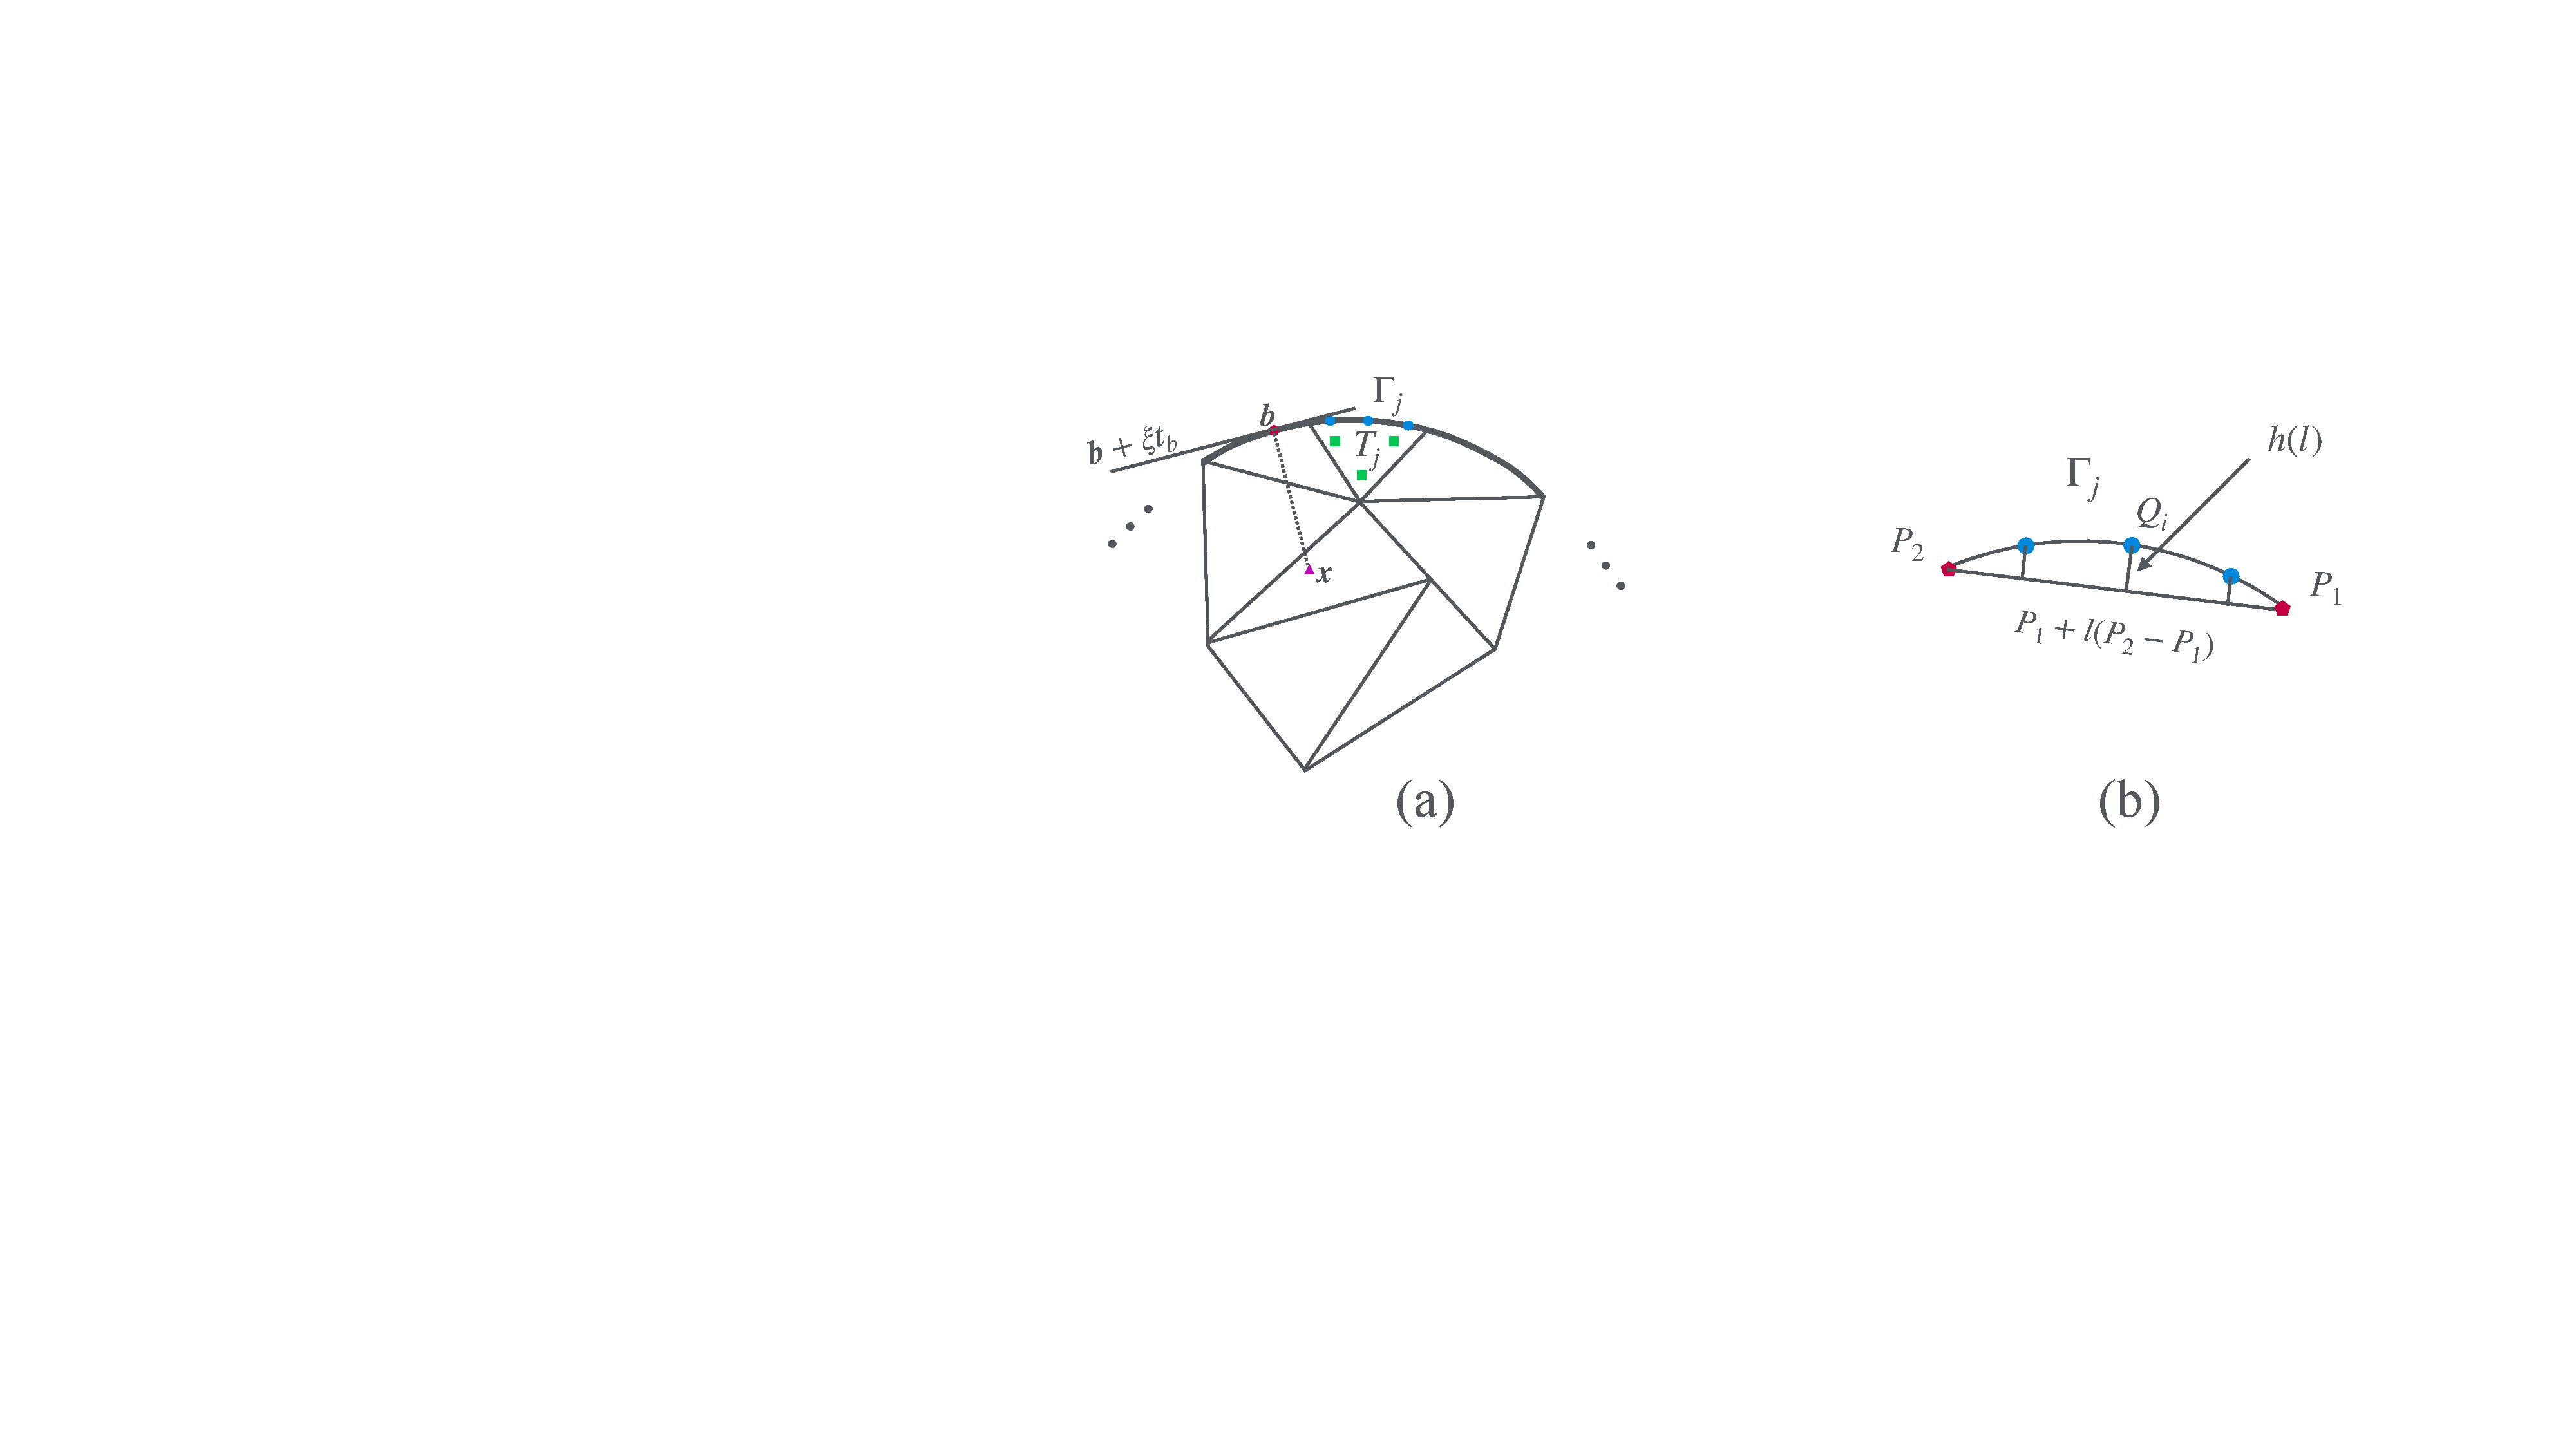
\includegraphics[width=0.78\textwidth]{fig-discrete_rev.pdf}
\end{frame}

% 18
\begin{frame}{FFT limitations for free-space potentials}
\small
The volume potential is a free-space convolution:
\[
  \Vop[f](\x)=\int_{\Omega}G(\x-\xp)f(\xp)\dd\xp.
\]

An ordinary FFT convolution on a box naturally gives a periodic convolution.

\begin{itemize}
  \item Periodic images alias the intended free-space Poisson solution.
  \item Zero padding helps but does not remove the singular quadrature issue.
  \item Unstructured points are not on a tensor grid.
\end{itemize}

\begin{block}{Relation to TKM and function extension}
\begin{itemize}
  \item Unlike TKM, where the computational domain is a cube, $\Omega$ here
  may have complex geometry.
  \item Unlike the function-extension approach, which uses an equispaced grid,
  $\Omega$ here is discretized by a triangulation or another unstructured mesh.
\end{itemize}
\end{block}
\end{frame}

% 19
\begin{frame}{Heat-equation representation}
\small
The key observation is that the Poisson volume potential is a steady-state
heat potential.

\[
  u_t(\x,t)-\Delta u(\x,t)=f(\x).
\]

With zero initial data at time $t=-\infty$, the solution at $t=0$ is
\[
  \Vop[f](\x)
  =
  \int_0^\infty\int_{\Omega}
  \frac{e^{-\|\x-\xp\|^2/4t}}{4\pi t}
  f(\xp)\dd\xp\dd t.
\]
\end{frame}

% 20
\begin{frame}{Heat semigroup derivation}
\small
In Fourier variables, the heat equation gives
\[
  \partial_t\widehat u(\kvec,t)+\|\kvec\|^2\widehat u(\kvec,t)=\widehat f(\kvec).
\]
The steady response from the infinite past is
\[
  \widehat u(\kvec,0)
  =
  \int_0^\infty e^{-\|\kvec\|^2t}\widehat f(\kvec)\dd t
  =
  \frac{\widehat f(\kvec)}{\|\kvec\|^2},
  \qquad \kvec\ne0.
\]

\vspace{1mm}
This coincides with the Poisson multiplier for $-\Delta u=f$.  The logarithmic
constant and zero mode are handled by the free-space Green's function convention.
\end{frame}

% 21
\begin{frame}{The heat kernel}
\small
In two dimensions,
\[
  K(\x,t)=\frac{e^{-\|\x\|^2/4t}}{4\pi t},\qquad t>0.
\]

\begin{itemize}
  \item For small $t$, $K$ is sharply localized in space.
  \item For large $t$, $K$ is broad and smooth.
  \item For every fixed $t>0$, $K$ is a smooth Gaussian.
\end{itemize}

\begin{block}{Kernel-split rationale}
Short time is local. Longer time is smooth enough for Fourier/NUFFT methods.
\end{block}
\end{frame}

% 22
\begin{frame}{Recovering the logarithm}
\small
For $\x\ne 0$,
\[
  \int_0^\delta
  \frac{e^{-\|\x\|^2/4t}}{4\pi t}\dd t
  =
  \frac{1}{4\pi}E_1\!\left(\frac{\|\x\|^2}{4\delta}\right),
\]
where $E_1$ is the exponential integral,
\[
  E_1(x)=\int_1^\infty \frac{e^{-tx}}{t}\dd t.
\]

Letting the upper limit go to infinity recovers the logarithmic Green's
function up to the usual additive constant.
\end{frame}

% 23
\begin{frame}{Asymptotics of the short-time kernel}
\small
Use the expansion
\[
  E_1(q)=-\gamma-\log q+q+\cO(q^2),
  \qquad q\to0.
\]
Here $\gamma$ is Euler's constant and $r=\|\x\|$.
With $q=r^2/(4\delta)$,
\[
  \frac{1}{4\pi}E_1\!\left(\frac{r^2}{4\delta}\right)
  =
  -\frac{1}{2\pi}\log r
  +
  \frac{1}{4\pi}\{\log(4\delta)-\gamma\}
  +\cO(r^2/\delta).
\]

The singular logarithm is already present in the short-time heat integral.
\end{frame}

% 24
\begin{frame}{Three-way heat split}
\small
Choose $0<\delta_1<\delta_2$. Then
\[
  \Vop[f]=\Vop_L[f]+\Vop_{NH}[f]+\Vop_{FH}[f],
\]
with
\[
\begin{aligned}
  \Vop_L[f]  &=\int_0^{\delta_1}\int_{\Omega}K(\x-\xp,t)f(\xp)\dd\xp\dd t,\\
  \Vop_{NH}[f]&=\int_{\delta_1}^{\delta_2}\int_{\Omega}K(\x-\xp,t)f(\xp)\dd\xp\dd t,\\
  \Vop_{FH}[f]&=\int_{\delta_2}^{\infty}\int_{\Omega}K(\x-\xp,t)f(\xp)\dd\xp\dd t.
\end{aligned}
\]
\end{frame}

% 25
\begin{frame}{Why split the history into near and far parts?}
\small
The local cutoff $\delta_1$ is small, so the history beginning at
$t=\delta_1$ still contains high Fourier frequencies.

\begin{itemize}
  \item On $\delta_1<t<\delta_2$, the near-history multiplier has a
  removable zero-mode singularity.  It is smooth and rapidly decaying, so
  this high-frequency contribution is handled directly by Fourier quadrature.

  \item On $t>\delta_2$, the Vico--Greengard--Ferrando truncated-kernel
  construction removes the zero-mode singularity, but its multiplier
  introduces additional oscillations.

  \item Omitting $\Vop_{NH}$ would require the far-history construction to
  begin at $\delta_1$.  The resulting one-level method costs approximately
  eight times the near-history component.
\end{itemize}

Choosing $\delta_2>8\delta_1$ moves the more oscillatory truncated-kernel
calculation to a smaller Fourier grid.  We use $\delta_2=32\delta_1$.
\end{frame}

% 24
\begin{frame}{Two-scale heat-kernel split}
\small
The logarithmic Green's function can be split as
\[
  G(\x)=G_H[\delta](\x)+G_L[\delta](\x),
\]
\[
  G_L[\delta](\x)=\frac{1}{4\pi}
  E_1\!\left(\frac{\|\x\|^2}{4\delta}\right),
\]
\[
  G_H[\delta](\x)=
  -\frac{1}{2\pi}\log\|\x\|
  -
  \frac{1}{4\pi}
  E_1\!\left(\frac{\|\x\|^2}{4\delta}\right).
\]

The heat-potential construction uses this identity to separate the local,
near-history, and far-history contributions at two time scales.
\end{frame}

% 25
\begin{frame}{Two-level implementation}
\small
\begin{itemize}
  \item We use a two-level algorithm for quasi-uniform volume
  discretizations, with $\delta_1=\cO(\Delta x^2)$, where $\Delta x$ is
  the average volume-node spacing.
  \item Near- and far-history Fourier integrals are evaluated by NUFFT sums on
  two different Fourier grids.
  \item The local contribution is evaluated by asymptotics and, when needed,
  dyadic correction.
\end{itemize}
\end{frame}

% 26
\begin{frame}{Fourier transform convention}
\small
Use
\[
  \hat f(\kvec)=
  \int_{\R^2}e^{-\ii\kvec\cdot\x}f(\x)\dd\x,
\]
and
\[
  f(\x)=\frac{1}{(2\pi)^2}
  \int_{\R^2}e^{\ii\kvec\cdot\x}\hat f(\kvec)\dd\kvec.
\]

The heat kernel has transform
\[
  \widehat{K(\cdot,t)}(\kvec)=e^{-\|\kvec\|^2t}.
\]

\vspace{1mm}
In the formulas below, the factor $(2\pi)^{-2}$ is shown in the analytic
representations and then absorbed into Fourier quadrature weights in the
algorithm slides.
\end{frame}

% 27
\begin{frame}{Near-history Fourier representation}
\small
By the convolution theorem and integration in time,
\[
  \Vop_{NH}[f](\x)
  =
  \frac{1}{(2\pi)^2}
  \int_{\R^2}
  \frac{
    e^{-\|\kvec\|^2\delta_1}
    -
    e^{-\|\kvec\|^2\delta_2}
  }{\|\kvec\|^2}
  e^{\ii\kvec\cdot\x}\hat f(\kvec)\dd\kvec.
\]

\begin{block}{Removable singularity}
The apparent singularity at $\kvec=0$ is removable.
\end{block}
\end{frame}

% 28
\begin{frame}{Near-history derivation}
\small
\[
\begin{aligned}
\Vop_{NH}[f](\x)
&=\int_{\delta_1}^{\delta_2}
  \left(K(\cdot,t)*f\right)(\x)\dd t\\
&=\frac{1}{(2\pi)^2}\int_{\delta_1}^{\delta_2}
  \int_{\R^2}
  e^{-\|\kvec\|^2t}
  e^{\ii\kvec\cdot\x}\hat f(\kvec)\dd\kvec\dd t\\
&=\frac{1}{(2\pi)^2}\int_{\R^2}
  \left(\int_{\delta_1}^{\delta_2}e^{-\|\kvec\|^2t}\dd t\right)
  e^{\ii\kvec\cdot\x}\hat f(\kvec)\dd\kvec.
\end{aligned}
\]
\[
  \int_{\delta_1}^{\delta_2}e^{-\|\kvec\|^2t}\dd t
  =
  \frac{e^{-\|\kvec\|^2\delta_1}-e^{-\|\kvec\|^2\delta_2}}
       {\|\kvec\|^2}.
\]
\end{frame}

% 29
\begin{frame}{Far-history accuracy in heat potentials}
\small
For $\delta_2<t<\infty$, the formal multiplier behaves like
\[
  \int_{\delta_2}^{\infty}e^{-\|\kvec\|^2t}\dd t
  =
  \frac{e^{-\|\kvec\|^2\delta_2}}{\|\kvec\|^2}.
\]

\begin{itemize}
  \item This has a nonintegrable-looking singularity at $\kvec=0$.
  \item The free-space Green's function also has infinite spatial support.
  \item The Vico-Greengard-Ferrando truncated-kernel method removes the singular
  behavior in a controlled way.
\end{itemize}
\end{frame}

% 30
\begin{frame}{Far-history free-space multiplier}
\small
Assume $f$ is supported in $\Omega\subset[-1,1]^2$ and targets lie in the
same box. The far history is approximated by
\[
  \Vop_{FH}[f](\x)
  \approx
  \frac{1}{(2\pi)^2}
  \int_{\R^2}
  e^{-\|\kvec\|^2\delta_2}
  W(\kvec)
  e^{\ii\kvec\cdot\x}\hat f(\kvec)\dd\kvec,
\]
where
\[
  W(\kvec)=
  \frac{1-J_0(2\sqrt2\,\|\kvec\|)}{\|\kvec\|^2}
  -
  \frac{2\sqrt2\log(2\sqrt2)\,J_1(2\sqrt2\,\|\kvec\|)}
       {\|\kvec\|}.
\]
Here $J_0$ and $J_1$ are Bessel functions of the first kind.
If the source support is distance $d$ from the boundary of the enclosing box,
the truncated-kernel replacement has error $\cO(e^{-d^2/\delta_2})$.
\end{frame}

% 31
\begin{frame}{Smoothness at the origin}
\small
Although $W(\kvec)$ is written with powers of $\|\kvec\|$ in the denominator,
Taylor expansion of the Bessel functions shows that $W$ is smooth at
$\kvec=0$.

\[
  \lim_{\|\kvec\|\to 0}W(\kvec)
  =
  \frac{(1-2\log(2\sqrt2))(2\sqrt2)^2}{4}.
\]

The Gaussian factor $e^{-\|\kvec\|^2\delta_2}$ supplies high-frequency
decay; the removable singularity does not require a special $\kvec=0$ rule.
\end{frame}

% 32
\begin{frame}{Layer history formulas}
\small
The same heat-potential representation works for layer potentials.
\[
  \Sop[\sigma]=\Sop_L[\sigma]+\Sop_{NH}[\sigma]+\Sop_{FH}[\sigma],
\]
\[
  \Dop[\mu]=\Dop_L[\mu]+\Dop_{NH}[\mu]+\Dop_{FH}[\mu].
\]

For example,
\[
  \Sop_{NH}[\sigma](\x)=
  \frac{1}{(2\pi)^2}
  \int_{\R^2}
  \frac{e^{-\|\kvec\|^2\delta_1}-e^{-\|\kvec\|^2\delta_2}}
       {\|\kvec\|^2}
  e^{\ii\kvec\cdot\x}\hat\sigma(\kvec)\dd\kvec.
\]
where
\[
  \hat\sigma(\kvec)=
  \int_{\partial\Omega}e^{-\ii\kvec\cdot\xp}\sigma(\xp)\dd s_{\xp}.
\]
\end{frame}

% 33
\begin{frame}{Double layer in Fourier space}
\small
For the near history of the double layer,
\[
\begin{aligned}
\Dop_{NH}[\mu](\x)
&=
\frac{1}{(2\pi)^2}
\int_{\R^2}
\frac{e^{-\|\kvec\|^2\delta_1}-e^{-\|\kvec\|^2\delta_2}}
     {\|\kvec\|^2}
e^{\ii\kvec\cdot\x} \\
&\qquad\qquad\cdot
\left[
\ii k_1\widehat{\mu\nu_1}(\kvec)
+\ii k_2\widehat{\mu\nu_2}(\kvec)
\right]\dd\kvec.
\end{aligned}
\]

\begin{block}{NUFFT inputs}
Volume and single layer sources require one transform. The double layer needs
normal-weighted boundary sources.
\end{block}

\[
  \widehat{\mu\nu_i}(\kvec)=
  \int_{\partial\Omega}e^{-\ii\kvec\cdot\xp}
  \mu(\xp)\nu_i(\xp)\dd s_{\xp},\qquad i=1,2.
\]
\end{frame}

% 34
\begin{frame}{Truncation in Fourier space}
\small
For a requested history tolerance $\epsilon>0$, choose cutoffs for volume and
single-layer terms so that
\[
  e^{-(k^{NH}_{\max})^2\delta_1}<\epsilon,
  \qquad
  e^{-(k^{FH}_{\max})^2\delta_2}<\epsilon.
\]
For double-layer terms, the corresponding tests include the derivative factor:
\[
  k^{NH}_{\max}e^{-(k^{NH}_{\max})^2\delta_1}<\epsilon,
  \qquad
  k^{FH}_{\max}e^{-(k^{FH}_{\max})^2\delta_2}<\epsilon.
\]

Then discretize the square Fourier boxes
\[
  [-k^{NH}_{\max},k^{NH}_{\max}]^2,
  \qquad
  [-k^{FH}_{\max},k^{FH}_{\max}]^2.
\]

\begin{itemize}
  \item Source points need not lie on a grid.
  \item Fourier modes do lie on a grid.
  \item This is the setting for a nonuniform FFT.
\end{itemize}
\end{frame}

% 35
\begin{frame}{Choosing $\delta_1$ and $\delta_2$}
\small
For quasi-uniform triangles, set
\[
  \delta_1=C\Delta x^2,
  \qquad C\approx 3.
\]
We take
\[
  \delta_2=32\delta_1
\]
in practice.

\begin{block}{Length scale}
$\sqrt{\delta_1}$ is proportional to the local mesh scale. The local part
is confined to a narrow band around each target or boundary chunk.
\end{block}
\end{frame}

% 36
\begin{frame}{Fourier mode estimates}
\small
If $N$ is the number of quasi-uniform volume nodes, then
$\Delta x=\cO(N^{-1/2})$ and $\delta_1=\cO(N^{-1})$.

With the approximately twice-Nyquist Fourier sampling used in the algorithm,
let $n_f^{NH}$ denote the number of nodes in each Fourier direction.  The
near-history grid has
\[
  n_f^{NH}
  \approx
  \frac{2\sqrt{\log(1/\epsilon)}}{\pi\sqrt{\delta_1}}
  =
  \cO(\sqrt N).
\]
So the total number of Fourier modes is
\[
  N_f^{NH}=(n_f^{NH})^2=\cO(N).
\]
\end{frame}

% 37
\begin{frame}{Accuracy and dyadic refinement}
\small
The local expansion uses $\delta_1=\cO(\Delta x^2)$.  A local-expansion
remainder of $\cO(\delta_1^{5/2})$ gives fifth-order accuracy in $\Delta x$.

\vspace{1mm}
In the reported third-order experiments, the expansions retain terms through
$\cO(\delta)$ and have remainders $\cO(\delta^{3/2})$.  Three levels of dyadic
refinement reduce the local layer-potential error.  With
\[
  \delta^\ast=\frac{\delta_1}{4^J},
\]
only the innermost interval $[0,\delta^\ast]$ uses the local asymptotic
formula; the remaining dyadic intervals use smooth difference kernels.
\end{frame}

% 38
\begin{frame}{NUFFT history algorithm: inputs}
\small
Given:
\begin{itemize}
  \item volume nodes $\x[j]$, weights $w[j]$, and source values $f(\x[j])$;
  \item boundary nodes $\x_\Gamma[j]$, weights $w_\Gamma[j]$;
  \item layer densities $\sigma(\x_\Gamma[j])$, $\mu(\x_\Gamma[j])$;
  \item normals $\nu_1,\nu_2$ on the boundary;
  \item target points anywhere in the enclosing box.
\end{itemize}

The history terms are evaluated by source-to-Fourier and Fourier-to-target NUFFTs.
\end{frame}

% 39
\begin{frame}{NUFFT history algorithm: grids}
\small
Build two Fourier grids.  Let $n_f^{NH}$ and $n_f^{FH}$ be the numbers of
nodes in each Fourier direction, and let
$N_f^{NH}=(n_f^{NH})^2$, $N_f^{FH}=(n_f^{FH})^2$.
\[
  \kvec_l^{NH}\in[-k_{\max}^{NH},k_{\max}^{NH}]^2,
  \qquad
  \kvec_l^{FH}\in[-k_{\max}^{FH},k_{\max}^{FH}]^2.
\]

The grid sizes are chosen using
\[
  n_f^{NH}
  =
  \frac{2\sqrt{\log(1/\epsilon)}}{\pi\sqrt{\delta_1}},
  \qquad
  n_f^{FH}
  =
  \frac{4\sqrt2\sqrt{\log(1/\epsilon)}}{\pi\sqrt{\delta_2}}.
\]
\end{frame}

% 40
\begin{frame}{NUFFT history algorithm: source to mode}
\small
For either Fourier grid $\{\kvec_l\}_{l=1}^{N_f}$, accumulate
\[
\begin{aligned}
\hat u[l]
&=
\sum_{j=1}^{N} e^{\ii\kvec_l\cdot \x[j]} f(\x[j])w[j]\\
&\quad+
\sum_{j=1}^{N_B} e^{\ii\kvec_l\cdot \x_\Gamma[j]}
\sigma(\x_\Gamma[j])w_\Gamma[j]\\
&\quad+
\ii k_{l,1}\sum_{j=1}^{N_B} e^{\ii\kvec_l\cdot \x_\Gamma[j]}
\mu(\x_\Gamma[j])\nu_1(\x_\Gamma[j])w_\Gamma[j]\\
&\quad+
\ii k_{l,2}\sum_{j=1}^{N_B} e^{\ii\kvec_l\cdot \x_\Gamma[j]}
\mu(\x_\Gamma[j])\nu_2(\x_\Gamma[j])w_\Gamma[j].
\end{aligned}
\]
\end{frame}

% 41
\begin{frame}{NUFFT history algorithm: mode to target}
\small
At a target $\x$, use the near multiplier
\[
  M_{NH}(\kvec)=
  \frac{e^{-\|\kvec\|^2\delta_1}-e^{-\|\kvec\|^2\delta_2}}
       {\|\kvec\|^2}
\]
and the far multiplier
\[
  M_{FH}(\kvec)=W(\kvec)e^{-\|\kvec\|^2\delta_2}.
\]
Then
\[
  u^{NH}(\x)=\sum_l \hat u_{NH}[l]M_{NH}(\kvec_l)e^{-\ii\kvec_l\cdot\x},
\]
\[
  u^{FH}(\x)=\sum_l \hat u_{FH}[l]M_{FH}(\kvec_l)e^{-\ii\kvec_l\cdot\x}.
\]

\vspace{1mm}
The source sum on the preceding slide is evaluated separately on the near and
far grids to obtain $\hat u_{NH}$ and $\hat u_{FH}$.  The discrete Fourier
quadrature weights, including $(2\pi)^{-2}$ and the mode spacing, are folded
into the multipliers.
\end{frame}

% 42
\begin{frame}{History complexity}
\small
Let $N_f^{NH}$ and $N_f^{FH}$ denote the total numbers of Fourier modes on
the near- and far-history grids, respectively, and let $N_{tot}$ be the total
number of target points.  The NUFFT cost is
\[
  \cO\!\left(N_f^{NH}\log N_f^{NH}+N_{tot}\right)
  +
  \cO\!\left(N_f^{FH}\log N_f^{FH}+N_{tot}\right).
\]

\begin{itemize}
  \item For a quasi-uniform volume discretization with $N$ interior points,
  $N_f^{NH}=\cO(N)$.
  \item When $\delta_2>8\delta_1$, the far-history grid has fewer Fourier
  modes than the near-history grid.
  \item Volume and single-layer contributions require one NUFFT call;
  double-layer contributions require two.
\end{itemize}
\end{frame}

% 43
\begin{frame}{Local heat potentials}
\small
The local contributions $\Vop_L$, $\Sop_L$, and $\Dop_L$ are the heat
integrals over $0<t<\delta_1$.  Their spatial scale is set by
\[
  e^{-\|\x-\xp\|^2/(4t)}.
\]

\begin{block}{Local-asymptotics threshold}
We assume $\delta_1$ is small enough that an interior target within
$12\sqrt{\delta_1}$ has a unique closest boundary point. The cutoff $12$ is
chosen because the local heat kernel has decayed below $10^{-14}$ at that
distance.
\end{block}
\end{frame}

% 44
\begin{frame}{Local coordinates near the boundary}
\small
Let $\bm b$ be the closest boundary point to $\x$, let $\nuvec_b$ be the
outward normal at $\bm b$, and set $r=\|\x-\bm b\|$, $\delta=\delta_1$,
and $c=r/\sqrt\delta$.  Use tangent-normal coordinates $(\xi,\eta)$ at
$\bm b$.

\[
  s(\x)=
  \begin{cases}
  1,&\x\in\Omega,\\
  0,&\x\in\partial\Omega,\\
  -1,&\x\in\Omega^E,
  \end{cases}
  \qquad
  \x=\bm b-s(\x)r\nuvec_b.
\]

The boundary has the local expansion
\[
  \eta=\gamma(\xi)
  =
  \frac12\kappa_b\xi^2
  +
  \frac16\gamma_b^{(3)}\xi^3
  +
  \frac1{24}\gamma_b^{(4)}\xi^4+\cdots,
\]
where $\kappa_b=\gamma''(0)$ is the boundary curvature.  For a density $h$,
$h_b=h(\bm b)$ and primes denote derivatives with respect to $\xi$ at $\bm b$.
\end{frame}

% 45
\begin{frame}{Where the local expansion comes from}
\small
For $0<t<\delta$, the heat kernel samples a neighborhood of diameter
$\cO(\sqrt\delta)$.  In the local heat integrals, set
\[
  z=\sqrt{4t},\qquad u=\frac{\xi}{z}.
\]
Taylor expanding $\gamma(\xi)$ and the density about $\bm b$, then integrating
the resulting Gaussian moments, gives the coefficients involving
$e^{-c^2/4}$ and $\erfc(c/2)$.
\end{frame}

% 46
\begin{frame}{Local single layer asymptotic}
\small
Keeping terms through $\cO(\delta)$, with $\delta=\delta_1$ and
$\x=\bm b-sr\nuvec_b$,
\[
\begin{aligned}
\Sop_L[\sigma](\x)
&=
\sqrt{\delta}\frac{\sigma_b}{2}
\left(
c\,\erfc\left(\frac c2\right)
-
\frac{2e^{-c^2/4}}{\sqrt\pi}
\right)\\
&\quad+
s\delta\frac{c\kappa_b\sigma_b}{4}
\left(
c\,\erfc\left(\frac c2\right)
-
\frac{2e^{-c^2/4}}{\sqrt\pi}
\right)
+\cO(\delta^{3/2}).
\end{aligned}
\]

\begin{block}{Observation}
The formula is uniform as the target approaches the boundary.
\end{block}
\end{frame}

% 46
\begin{frame}{Local double layer asymptotic}
\scriptsize
Here $\x=\bm b-sr\nuvec_b$, where $s=s(\x)$ specifies the side of the
boundary.
\[
\begin{aligned}
\Dop_L[\mu](\x)
&=
s\frac{\mu_b}{2}
\erfc\left(\frac c2\right)
+\sqrt{\delta}\frac{\kappa_b\mu_b}{2\sqrt\pi}e^{-c^2/4}\\
&\quad+
\delta\,s
\left[
\frac{3c\kappa_b^2\mu_b}{8\sqrt\pi}e^{-c^2/4}
+
\frac{c\mu_b''}{4}
\left(
\frac{2e^{-c^2/4}}{\sqrt\pi}
-
c\,\erfc\left(\frac c2\right)
\right)
\right]
+\cO(\delta^{3/2}).
\end{aligned}
\]

\end{frame}

% 47
\begin{frame}{Local volume asymptotic}
\small
For a target inside $\Omega$ near the boundary,
\[
  \Vop_L[f](\x)
  =
  \frac{\delta}{4}
  \left(
  2\erf\left(\frac c2\right)
  +
  \frac{2e^{-c^2/4}c}{\sqrt\pi}
  -
  c^2\erfc\left(\frac c2\right)
  +2
  \right)f
  +
  \cO(\delta^{3/2}).
\]
Here $f=f(\x)$ is the source density at the target.

\begin{block}{Away from the boundary}
When exponentially small boundary terms are negligible,
\[
  \Vop_L[f](\x)=\delta f+\frac{\delta^2}{2}\Delta f+\cO(\delta^3).
\]
\end{block}
\end{frame}

% 48
\begin{frame}{Boundary simplification}
\small
For target points on $\partial\Omega$, the volume local term simplifies to
\[
  \Vop_L[f](\x)
  =
  \frac{\delta}{2}f
  +
  \frac{\delta^{3/2}}{3\sqrt\pi}
  \left(2f_\eta-\kappa_b f\right)
  +
  \frac{\delta^2}{4}\left(f_{\xi\xi}+f_{\eta\eta}\right)
  +
  \cO(\delta^{5/2}).
\]
The derivatives are evaluated at the target; $\xi$ is tangential and $\eta$ is
the inward normal direction.

\begin{itemize}
  \item Boundary evaluations are needed for the BIE right-hand side.
  \item Curvature enters through the local asymptotics.
  \item Higher order terms require higher derivatives and are less robust.
\end{itemize}
\end{frame}

% 49
\begin{frame}{Telescoping local correction}
\small
If the asymptotic order is not enough, do not shrink $\delta_1$ globally.
That would enlarge the NUFFT grids.

Instead choose $J$ so that
\[
  \left(\frac{\delta_1}{4^J}\right)^p\le \epsilon,
  \qquad
  \delta^\ast=\frac{\delta_1}{4^J}.
\]

Then split
\[
  [0,\delta_1]
  =
  [0,\delta^\ast]
  \cup
  \bigcup_{j=1}^J
  \left[\frac{\delta_1}{4^j},\frac{\delta_1}{4^{j-1}}\right].
\]
\end{frame}

% 50
\begin{frame}{Difference kernels}
\small
For the single layer local part, the dyadic pieces use smooth kernels
\[
  \Kop_j(q)
  =
  \frac{1}{4\pi}
  \left[
  E_1(4^{j-2}q)-E_1(4^{j-1}q)
  \right].
\]
where $q=\|\x-\xp\|^2/\delta_1$.

\begin{itemize}
  \item The $[0,\delta^\ast]$ piece is handled by asymptotics.
  \item The dyadic pieces are evaluated by smooth local quadrature.
  \item The interaction range shrinks by a factor of two per level.
\end{itemize}
\end{frame}

% 51
\begin{frame}{Cost of dyadic close-history corrections}
\small
At level $j$, the heat interval has effective spatial radius
\[
  r_j\sim \sqrt{\delta_1/4^j}=2^{-j}\sqrt{\delta_1}.
\]
At each level, the interaction range halves while the required local spatial
resolution doubles.  Thus the number of source nodes that contribute
non-negligibly to a target remains approximately unchanged from level to level.

\begin{block}{Important distinction}
Dyadic correction refines only the local physical-space quadrature.  It does not
change $k_{\max}^{NH}$ or the global NUFFT grids.
\end{block}
\end{frame}

% 52
\begin{frame}{Boundary integral correction}
\small
After the volume potential is available, solve a classical BIE.

Interior Dirichlet:
\[
  -\frac12\mu+\Dop[\mu]
  =
  g-\Vop[f]
  \quad\text{on }\partial\Omega.
\]

Interior Neumann:
\[
  \frac12 u+\Dop[u]
  =
  \Vop[f]+\Sop[g]
  \quad\text{on }\partial\Omega.
\]

\begin{block}{Implementation}
We use GMRES with FMM acceleration for the BIE, and FINUFFT for
history evaluation.
\end{block}
\end{frame}

% 52
\begin{frame}{Validation of local asymptotics}
\centering
\begin{columns}[T,totalwidth=\textwidth]
\begin{column}{0.48\textwidth}
\resizebox{\textwidth}{!}{% This file was created by matlab2tikz.
%
%The latest updates can be retrieved from
%  http://www.mathworks.com/matlabcentral/fileexchange/22022-matlab2tikz-matlab2tikz
%where you can also make suggestions and rate matlab2tikz.
%
\definecolor{mycolor1}{rgb}{0.00000,0.44700,0.74100}%
\definecolor{mycolor2}{rgb}{0.85000,0.32500,0.09800}%
%
\begin{tikzpicture}[scale=0.55]

\begin{axis}[%
%width=4.602in,
%height=3.743in,
%at={(0.772in,0.593in)},
scale only axis,
xmode=log,
xmin=0.000001,
xmax=0.003,
xminorticks=true,
xlabel style={font=\Large\color{white!15!black}},
xlabel={$\delta$},
xticklabel style = {font=\large},
extra x ticks={0.002},
extra x tick labels={},
ymode=log,
ymin=1e-12,
ymax=0.001,
yminorticks=true,
ylabel style={font=\Large\color{white!15!black}},
ylabel={Relative error},
yticklabel style = {font=\large},
axis background/.style={fill=white},
xmajorgrids,
xminorgrids,
ymajorgrids,
yminorgrids,
legend style={font=\Large,at={(0.03,0.97)}, anchor=north west, legend cell align=left, align=left, draw=white!15!black},
clip mode=individual,
]
%%%%%%%%%%%%%%%%%% delta^(4/2) %%%%%%%%%%%%%%%%%%
\addplot [color=mycolor1, line width=1.0pt, mark=square*, mark options={solid, mycolor1}, mark size=2.0pt]
  table[row sep=crcr]{%
1.000000e-03 6.965999e-04 \\
5.274997e-04 1.820020e-04 \\
2.782559e-04 5.289530e-05 \\
1.467799e-04 1.325988e-05 \\
7.742637e-05 2.732296e-06 \\
4.084239e-05 8.285891e-07 \\
2.154435e-05 2.349053e-07 \\
1.136464e-05 5.610848e-08 \\
5.994843e-06 1.137074e-08 \\
3.162278e-06 3.068346e-09 \\
};
%\addlegendentry{$e_{\infty}$}

\addplot [color=mycolor2, dotted, line width=1.0pt, mark=square, mark options={solid, mycolor2}, mark size=2.0pt]
  table[row sep=crcr]{%
1.000000e-03 8.691356e-05 \\
5.274997e-04 2.011701e-05 \\
2.782559e-04 4.696373e-06 \\
1.467799e-04 1.106289e-06 \\
7.742637e-05 2.567208e-07 \\
4.084239e-05 6.054419e-08 \\
2.154435e-05 1.434273e-08 \\
1.136464e-05 3.511387e-09 \\
5.994843e-06 8.152016e-10 \\
3.162278e-06 1.663777e-10 \\
};
%\addlegendentry{$e_{2}$}

\addplot [color=black, dashed, line width=1.0pt]
  table[row sep=crcr]{%
%1.000000e-03 9.205038e-04 \\
%5.274997e-04 2.561356e-04 \\
%2.782559e-04 7.127127e-05 \\
%1.467799e-04 1.983165e-05 \\
7.742637e-05 5.518275e-06 \\
4.084239e-05 1.535493e-06 \\
2.154435e-05 4.272600e-07 \\
1.136464e-05 1.188876e-07 \\
5.994843e-06 3.308119e-08 \\
%3.162278e-06 9.205038e-09 \\
};
%\addlegendentry{$O(\Delta x^{2})$}
%%%%%%%%%%%%%%%%%% delta^(5/2) %%%%%%%%%%%%%%%%%%
\addplot [color=mycolor1, line width=1.0pt, mark=*, mark options={solid, mycolor1}, mark size=2.0pt]
  table[row sep=crcr]{%
1.000000e-03 4.717426e-04 \\
5.274997e-04 1.158198e-04 \\
2.782559e-04 2.247010e-05 \\
1.467799e-04 5.795497e-06 \\
7.742637e-05 1.223693e-06 \\
4.084239e-05 1.939333e-07 \\
2.154435e-05 4.498951e-08 \\
1.136464e-05 1.003251e-08 \\
5.994843e-06 1.962563e-09 \\
3.162278e-06 2.810016e-10 \\
};
%\addlegendentry{$e_{\infty}$}

\addplot [color=mycolor2, dotted, line width=1.0pt, mark=o, mark options={solid, mycolor2}, mark size=2.0pt]
  table[row sep=crcr]{%
1.000000e-03 5.478049e-05 \\
5.274997e-04 1.086689e-05 \\
2.782559e-04 2.014275e-06 \\
1.467799e-04 3.671940e-07 \\
7.742637e-05 6.877565e-08 \\
4.084239e-05 1.228032e-08 \\
2.154435e-05 2.136913e-09 \\
1.136464e-05 3.882554e-10 \\
5.994843e-06 6.840687e-11 \\
3.162278e-06 1.012669e-11 \\
};
%\addlegendentry{$e_{2}$}

\addplot [color=black, dashdotdotted, line width=1.0pt]
  table[row sep=crcr]{%
%1.000000e-03 7.203235e-05 \\
%5.274997e-04 1.455738e-05 \\
%2.782559e-04 2.941973e-06 \\
%1.467799e-04 5.945581e-07 \\
7.742637e-05 1.201572e-07 \\
4.084239e-05 2.428317e-08 \\
2.154435e-05 4.907507e-09 \\
1.136464e-05 9.917826e-10 \\
5.994843e-06 2.004343e-10 \\
%3.162278e-06 4.050677e-11 \\
};
%\addlegendentry{$O(\Delta x ^{3})$}
\end{axis}


\end{tikzpicture}%
%%% Local Variables:
%%% mode: latex
%%% TeX-master: ../poissongaussfryk.tex
%%% End:
}
\end{column}
\begin{column}{0.48\textwidth}
\resizebox{\textwidth}{!}{% This file was created by matlab2tikz.
%
%The latest updates can be retrieved from
%  http://www.mathworks.com/matlabcentral/fileexchange/22022-matlab2tikz-matlab2tikz
%where you can also make suggestions and rate matlab2tikz.
%
\definecolor{mycolor1}{rgb}{0.00000,0.44700,0.74100}%
\definecolor{mycolor2}{rgb}{0.85000,0.32500,0.09800}%
%
\begin{tikzpicture}[scale=0.55]

\begin{axis}[%
%width=4.602in,
%height=3.743in,
%at={(0.772in,0.593in)},
scale only axis,
xmode=log,
xmin=0.000001,
xmax=0.003,
xminorticks=true,
xlabel style={font=\Large\color{white!15!black}},
xlabel={$\delta$},
xticklabel style = {font=\large},
extra x ticks={0.002},
extra x tick labels={},
ymode=log,
ymin=1e-10,
ymax=0.01,
yminorticks=true,
ylabel style={font=\Large\color{white!15!black}},
ylabel={Relative error},
yticklabel style = {font=\large},
axis background/.style={fill=white},
xmajorgrids,
xminorgrids,
ymajorgrids,
yminorgrids,
legend style={font=\Large,at={(0.03,0.97)}, anchor=north west, legend cell align=left, align=left, draw=white!15!black},
clip mode=individual,
]
%%%%%%%%%%%%%%%%%% delta^(4/2) %%%%%%%%%%%%%%%%%%
\addplot [color=mycolor1, line width=1.0pt, mark=square*, mark options={solid, mycolor1}, mark size=2.0pt]
  table[row sep=crcr]{%
1.000000e-03 1.167069e-02 \\
5.274997e-04 3.423291e-03 \\
2.782559e-04 8.917484e-04 \\
1.467799e-04 1.939171e-04 \\
7.742637e-05 7.029816e-05 \\
4.084239e-05 1.748774e-05 \\
2.154435e-05 4.062158e-06 \\
1.136464e-05 1.517986e-06 \\
5.994843e-06 4.576037e-07 \\
3.162278e-06 1.000210e-07 \\
};
%\addlegendentry{$e_{\infty}$}

\addplot [color=mycolor2, dotted, line width=1.0pt, mark=square, mark options={solid, mycolor2}, mark size=2.0pt]
  table[row sep=crcr]{%
1.000000e-03 1.045028e-03 \\
5.274997e-04 2.663575e-04 \\
2.782559e-04 6.385036e-05 \\
1.467799e-04 1.496642e-05 \\
7.742637e-05 3.819651e-06 \\
4.084239e-05 9.642586e-07 \\
2.154435e-05 2.337636e-07 \\
1.136464e-05 5.984352e-08 \\
5.994843e-06 1.495002e-08 \\
3.162278e-06 3.186447e-09 \\
};
%\addlegendentry{$e_{2}$}

\addplot [color=black, dashed, line width=1.0pt]
  table[row sep=crcr]{%
%1.000000e-03 2.000420e-02 \\
%5.274997e-04 5.566289e-03 \\
%2.782559e-04 1.548853e-03 \\
%1.467799e-04 4.309775e-04 \\
7.742637e-05 1.199221e-04 \\
4.084239e-05 3.336902e-05 \\
2.154435e-05 9.285129e-06 \\
1.136464e-05 2.583642e-06 \\
5.994843e-06 7.189138e-07 \\
%3.162278e-06 2.000420e-07 \\
};
%\addlegendentry{$O(\Delta x^{2})$}
%%%%%%%%%%%%%%%%%% delta^(5/2) %%%%%%%%%%%%%%%%%%
\addplot [color=mycolor1, line width=1.0pt, mark=*, mark options={solid, mycolor1}, mark size=2.0pt]
  table[row sep=crcr]{%
 1.000000e-03 1.224455e-02 \\
5.274997e-04 3.027073e-03 \\
2.782559e-04 6.410129e-04 \\
1.467799e-04 1.431911e-04 \\
7.742637e-05 2.968500e-05 \\
4.084239e-05 5.639604e-06 \\
2.154435e-05 9.383464e-07 \\
1.136464e-05 1.179222e-07 \\
5.994843e-06 1.465262e-08 \\
3.162278e-06 2.722173e-09 \\
};
%\addlegendentry{$e_{\infty}$}

\addplot [color=mycolor2, dotted, line width=1.0pt, mark=o, mark options={solid, mycolor2}, mark size=2.0pt]
  table[row sep=crcr]{%
1.000000e-03 9.060404e-04 \\
5.274997e-04 1.867084e-04 \\
2.782559e-04 3.828869e-05 \\
1.467799e-04 7.214800e-06 \\
7.742637e-05 1.222515e-06 \\
4.084239e-05 2.122962e-07 \\
2.154435e-05 3.691164e-08 \\
1.136464e-05 5.502208e-09 \\
5.994843e-06 7.691716e-10 \\
3.162278e-06 1.422768e-10 \\
};
%\addlegendentry{$e_{2}$}

\addplot [color=black, dashdotdotted, line width=1.0pt]
  table[row sep=crcr]{%
%1.000000e-03 1.265039e-04 \\
%5.274997e-04 2.556581e-05 \\
%2.782559e-04 5.166723e-06 \\
%1.467799e-04 1.044169e-06 \\
7.742637e-05 2.110213e-07 \\
4.084239e-05 4.264634e-08 \\
2.154435e-05 8.618613e-09 \\
1.136464e-05 1.741778e-09 \\
5.994843e-06 3.520047e-10 \\
%3.162278e-06 7.113839e-11 \\
};
%\addlegendentry{$O(\Delta x ^{3})$}
\end{axis}


\end{tikzpicture}%
%%% Local Variables:
%%% mode: latex
%%% TeX-master: ../poissongaussfryk.tex
%%% End:
}
\end{column}
\end{columns}
\vspace{1mm}
\scriptsize
Local single- and double-layer errors as functions of $\delta$.
\end{frame}

% 53
\begin{frame}{Validation of the local volume expansion}
\centering
\resizebox{0.52\textwidth}{!}{% This file was created by matlab2tikz.
%
%The latest updates can be retrieved from
%  http://www.mathworks.com/matlabcentral/fileexchange/22022-matlab2tikz-matlab2tikz
%where you can also make suggestions and rate matlab2tikz.
%
\definecolor{mycolor1}{rgb}{0.00000,0.44700,0.74100}%
\definecolor{mycolor2}{rgb}{0.85000,0.32500,0.09800}%
%
\begin{tikzpicture}[scale=0.55]

\begin{axis}[%
%width=4.602in,
%height=3.743in,
%at={(0.772in,0.593in)},
scale only axis,
xmode=log,
xmin=0.000001,
xmax=0.003,
xminorticks=true,
xlabel style={font=\Large\color{white!15!black}},
xlabel={$\delta$},
xticklabel style = {font=\large},
extra x ticks={0.002},
extra x tick labels={},
ymode=log,
ymin=1e-09,
ymax=1,
yminorticks=true,
ylabel style={font=\Large\color{white!15!black}},
ylabel={Relative error},
yticklabel style = {font=\large},
axis background/.style={fill=white},
xmajorgrids,
xminorgrids,
ymajorgrids,
yminorgrids,
legend style={font=\Large,at={(0.03,0.97)}, anchor=north west, legend cell align=left, align=left, draw=white!15!black},
clip mode=individual,
]
%%%%%%%%%%%%%%%%%% delta^(4/2) %%%%%%%%%%%%%%%%%%
\addplot [color=mycolor1, line width=1.0pt, mark=square*, mark options={solid, mycolor1}, mark size=2.0pt]
  table[row sep=crcr]{%
   0.000961644406940   0.052418548681328\\
   0.000541436243713   0.022276932315192\\
   0.000237951818000   0.005850522940774\\
   0.000060815169185   0.000480222684418\\
   0.000009763223090   0.000013409773430\\
   0.000005494895537   0.000004304253251\\
   0.000002443885747   0.000000857792870\\
};
%\addlegendentry{$e_{\infty}$}

\addplot [color=mycolor2, dotted, line width=1.0pt, mark=square, mark options={solid, mycolor2}, mark size=2.0pt]
  table[row sep=crcr]{%
   0.000961644406940   0.011835289670045\\
   0.000541436243713   0.005030375486929\\
   0.000237951818000   0.001294998964960\\
   0.000060815169185   0.000105142137848\\
   0.000009763223090   0.000002917722176\\
   0.000005494895537   0.000000930302648\\
   0.000002443885747   0.000000184887199\\
};
%\addlegendentry{$e_{2}$}

\addplot [color=black, dashed, line width=1.0pt]
  table[row sep=crcr]{%
%   0.000541436243713   0.095159793152161\\
   0.000237951818000   0.018379635559094\\
   0.000060815169185   0.001200556711046\\
   0.000009763223090   0.000030941778108\\
};
%\addlegendentry{$O(\Delta x^{2})$}
%%%%%%%%%%%%%%%%%% delta^(5/2) %%%%%%%%%%%%%%%%%%
\addplot [color=mycolor1, line width=1.0pt, mark=*, mark options={solid, mycolor1}, mark size=2.0pt]
  table[row sep=crcr]{%
   0.000961644406940   0.080967361355944\\
   0.000541436243713   0.019876793653893\\
   0.000237951818000   0.002274445795928\\
   0.000060815169185   0.000048753018903\\
   0.000009763223090   0.000000331566570\\
   0.000005494895537   0.000000088167434\\
   0.000002443885747   0.000000028095591\\
};
%\addlegendentry{$e_{\infty}$}

\addplot [color=mycolor2, dotted, line width=1.0pt, mark=o, mark options={solid, mycolor2}, mark size=2.0pt]
  table[row sep=crcr]{%
   0.000961644406940   0.017558435466307\\
   0.000541436243713   0.004308001782118\\
   0.000237951818000   0.000498894356057\\
   0.000060815169185   0.000010624205802\\
   0.000009763223090   0.000000056767682\\
   0.000005494895537   0.000000015391968\\
   0.000002443885747   0.000000003995063\\
};
%\addlegendentry{$e_{2}$}

\addplot [color=black, dashdotdotted, line width=1.0pt]
  table[row sep=crcr]{%
%   0.000541436243713   0.00028825711389979\\
   0.000237951818000   0.00003690917110281\\
   0.000060815169185   0.00000121882547258\\
   0.000009763223090   0.00000001258620371\\
};
%\addlegendentry{$O(\Delta x ^{3})$}
\end{axis}


\end{tikzpicture}%
%%% Local Variables:
%%% mode: latex
%%% TeX-master: ../poissongaussfryk.tex
%%% End:
}
\par\vspace{1mm}
\footnotesize
\parbox{0.82\textwidth}{\centering Local volume-potential error as a function of $\delta$.\par}
\end{frame}

% 53
\begin{frame}{Interior Neumann test geometry}
\centering
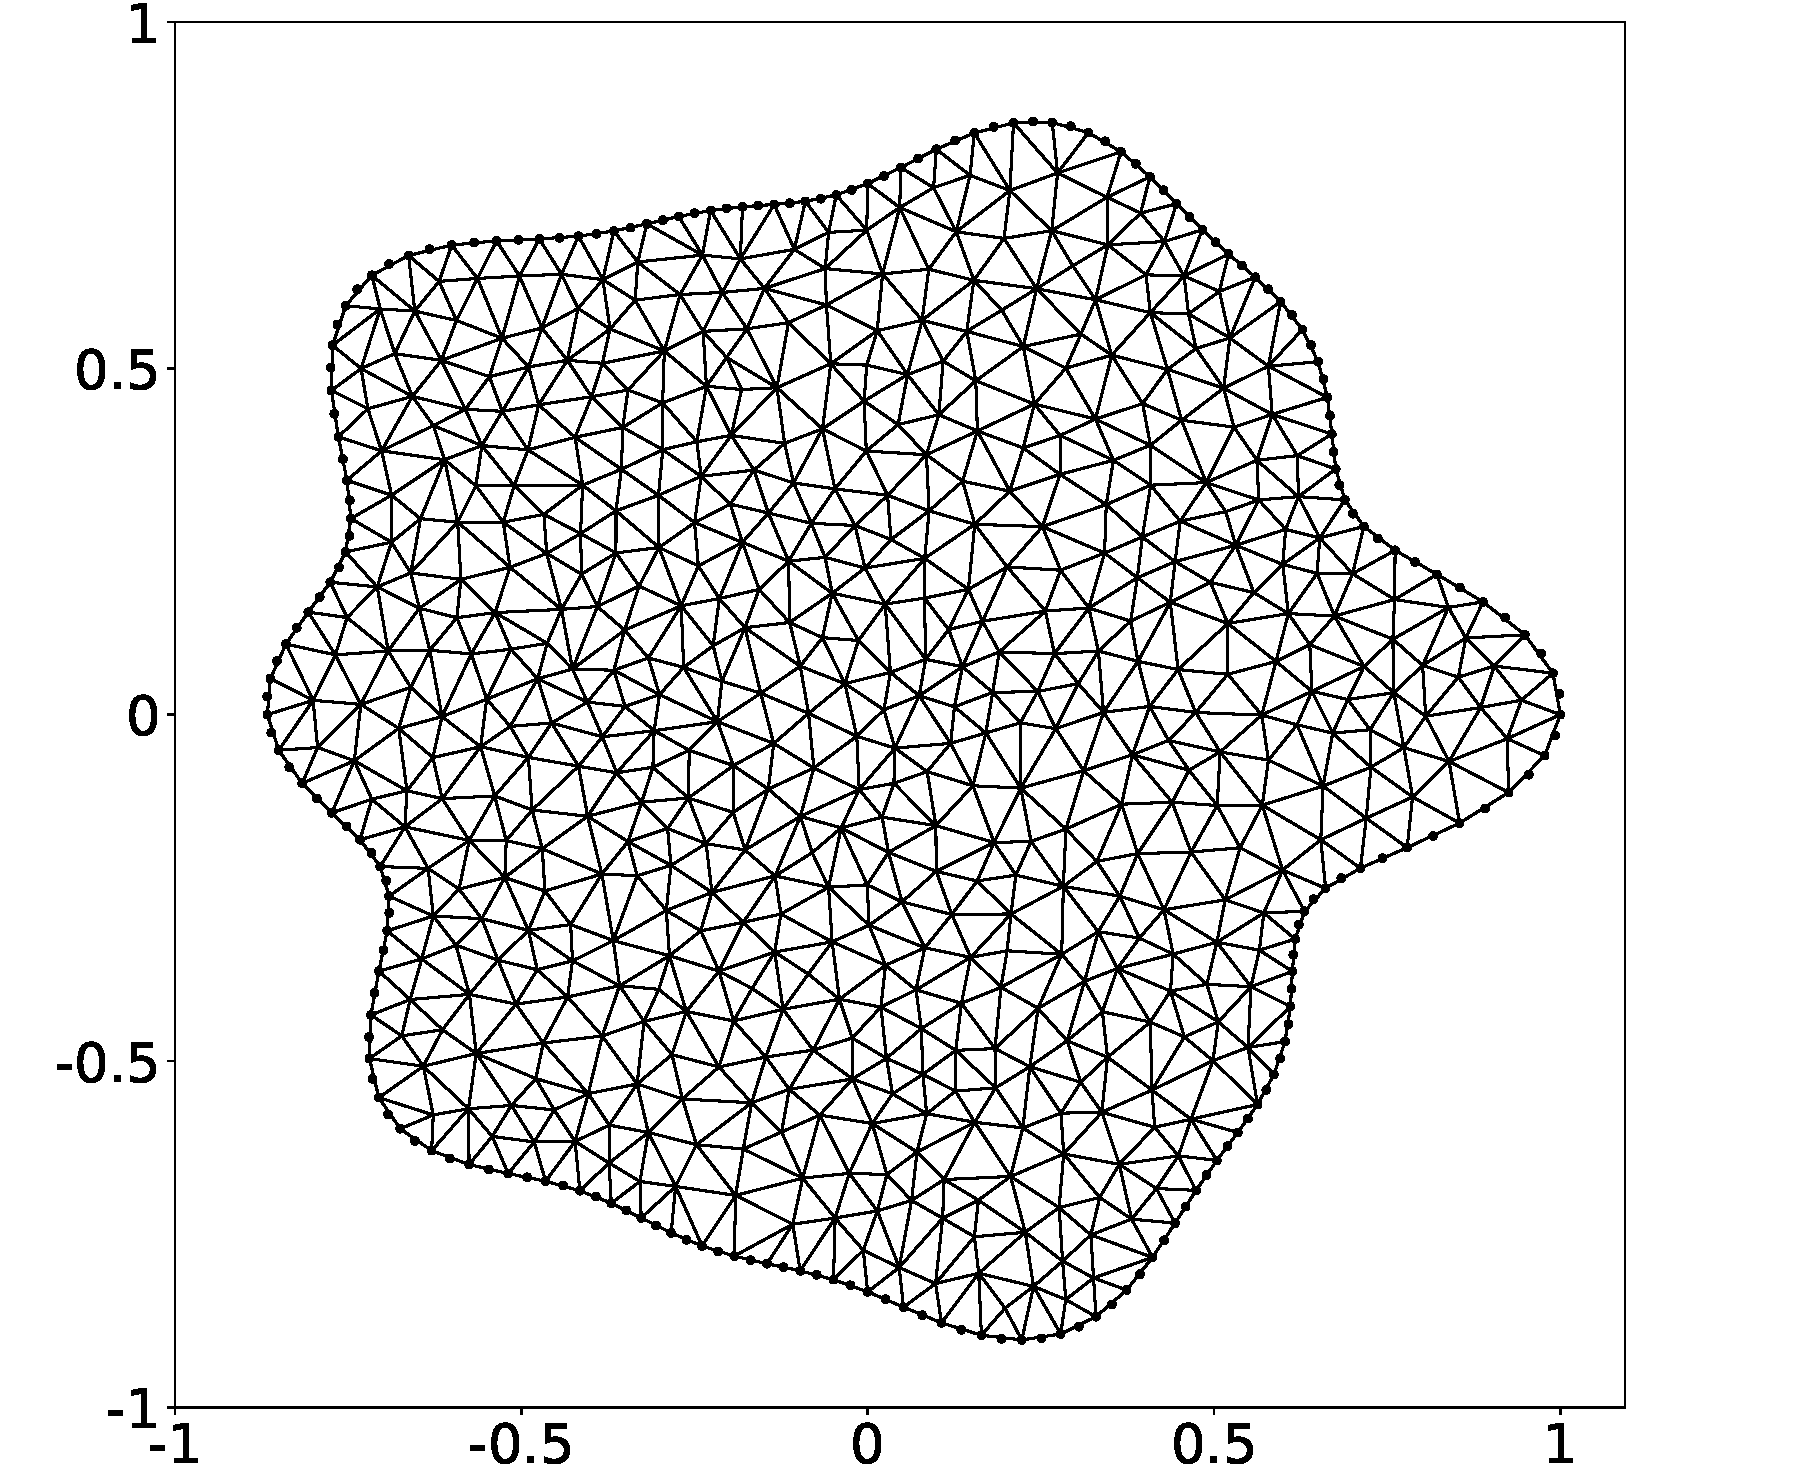
\includegraphics[height=0.66\textheight]{meshinth1_cropped.pdf}

\vspace{1mm}
\scriptsize
Quasi-uniform volumetric mesh for $\Omega$: 1142 triangles with $h\approx0.1$
and 208 boundary nodes.
\end{frame}

% 54
\begin{frame}{Interior Neumann errors and timing}
\centering
\begin{columns}[T,totalwidth=\textwidth]
\begin{column}{0.48\textwidth}
\resizebox{0.97\textwidth}{!}{% This file was created by matlab2tikz.
%
%The latest updates can be retrieved from
%  http://www.mathworks.com/matlabcentral/fileexchange/22022-matlab2tikz-matlab2tikz
%where you can also make suggestions and rate matlab2tikz.
%
\definecolor{mycolor1}{rgb}{0.00000,0.44700,0.74100}%
\definecolor{mycolor2}{rgb}{0.85000,0.32500,0.09800}%
%
\begin{tikzpicture}[scale=0.78]

\begin{axis}[%
%width=4.602in,
%height=3.743in,
%at={(0.772in,0.593in)},
scale only axis,
xmode=log,
xmin=0.0008,
xmax=0.03,
xminorticks=true,
xlabel style={font=\Large\color{white!15!black}},
xlabel={$\Delta x$},
xticklabel style = {font=\large},
extra x ticks={0.02},
extra x tick labels={},
ymode=log,
ymin=1e-05,
ymax=0.01,
yminorticks=true,
ylabel style={font=\Large\color{white!15!black}},
ylabel={Relative error},
yticklabel style = {font=\large},
axis background/.style={fill=white},
xmajorgrids,
xminorgrids,
ymajorgrids,
yminorgrids,
legend style={font=\Large,at={(0.03,0.97)}, anchor=north west, legend cell align=left, align=left, draw=white!15!black},
clip mode=individual,
]
\addplot [color=mycolor1, line width=1.0pt, mark=*, mark options={solid, mycolor1}, mark size=2.0pt]
  table[row sep=crcr]{%
0.01790385812183147018    0.00168410235516133376 \\
0.01343423789815931420    0.00078643877915392593 \\
0.00890602451526747822    0.00026105613355286263 \\
0.00450241302656924445    0.00003412405330157142 \\
0.00180399769861288597    0.00001613733264982419 \\
0.00135337793900323412    0.00001448728641231380 \\
0.00090256777153838587    0.00001388328731379843 \\
};
\addlegendentry{$e_{\infty}$}

\addplot [color=mycolor2, dotted, line width=1.0pt, mark=o, mark options={solid, mycolor2}, mark size=2.0pt]
  table[row sep=crcr]{%
0.01790385812183147018    0.00220041404519815851 \\
0.01343423789815931420    0.00108275239038070495 \\
0.00890602451526747822    0.00033572421149432382 \\
0.00450241302656924445    0.00003266028790814501 \\
0.00180399769861288597    0.00001503554273761145 \\
0.00135337793900323412    0.00001310721401032398 \\
0.00090256777153838587    0.00001267326524460375 \\
};
\addlegendentry{$e_{2}$}

\addplot [color=black, dashed, line width=1.0pt]
  table[row sep=crcr]{%
0.0179038581218315	0.00426996571900406\\
0.0134342378981593	0.0018039463170365\\
0.00890602451526748	0.000525576773152868\\
0.00450241302656925	6.79079315483874e-05\\
};
\addlegendentry{$O(\Delta x ^{3})$}

\end{axis}


\end{tikzpicture}%
%%% Local Variables:
%%% mode: latex
%%% TeX-master: ../poissongaussfryk.tex
%%% End:
}

\scriptsize Reported relative $\ell_\infty$ and $\ell_2$ errors; the dashed line is
$O(\Delta x^3)$.
\end{column}
\begin{column}{0.48\textwidth}
\resizebox{0.97\textwidth}{!}{% This file was created by matlab2tikz.
%
%The latest updates can be retrieved from
%  http://www.mathworks.com/matlabcentral/fileexchange/22022-matlab2tikz-matlab2tikz
%where you can also make suggestions and rate matlab2tikz.
%
\begin{tikzpicture}[scale=0.78]

\begin{axis}[%
%width=4.602in,
%height=3.743in,
%at={(0.772in,0.593in)},
scale only axis,
xmode=log,
xmin=1000,
xmax=10000000,
xminorticks=true,
xlabel style={font=\Large\color{white!15!black}},
xlabel={$N$},
xticklabel style = {font=\large},
ymode=log,
ymin=0.01,
ymax=10,
yminorticks=true,
ylabel style={font=\Large\color{white!15!black}},
ylabel={Time (sec)},
yticklabel style = {font=\large},
axis background/.style={fill=white},
scaled ticks=true
]
\addplot [color=black, line width=1.0pt, mark=o, mark options={solid, black}, forget plot]
  table[row sep=crcr]{%
6852    0.02998300000000142518 \\
12168    0.02721399999998652675 \\
27684    0.04241200000001299486 \\
108312    0.15037699999999176725 \\
674664    0.52396400000000653563 \\
1198728    0.87523499999998932708 \\
2695248    1.99756799999999401507 \\
};

\end{axis}

\end{tikzpicture}%
}

\scriptsize Total solve-and-evaluate time, excluding mesh generation.
\end{column}
\end{columns}
\end{frame}

% 55
\begin{frame}{Exterior Dirichlet geometry and error}
\small
\begin{columns}[T,totalwidth=\textwidth]
\begin{column}{0.48\textwidth}
\centering
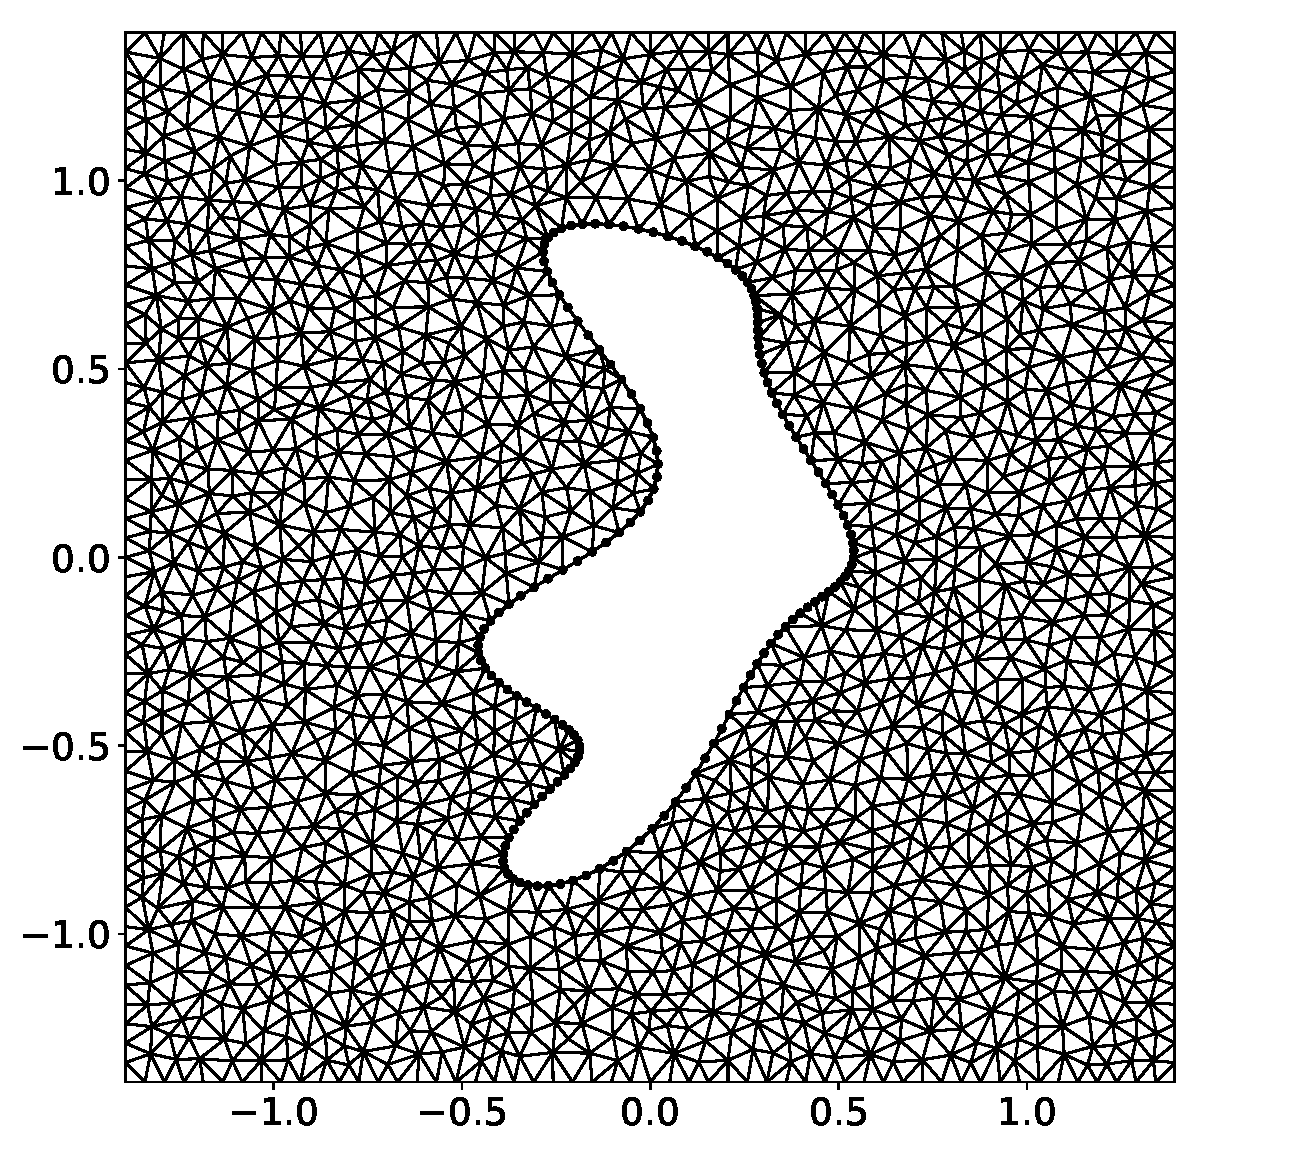
\includegraphics[width=\textwidth]{meshexth1_cropped.pdf}

\vspace{1mm}
\scriptsize Exterior-domain mesh on
$D=[-1.95,1.95]^2\setminus\overline\Omega$.
\end{column}
\begin{column}{0.48\textwidth}
\centering
\resizebox{\textwidth}{!}{% This file was created by matlab2tikz.
%
%The latest updates can be retrieved from
%  http://www.mathworks.com/matlabcentral/fileexchange/22022-matlab2tikz-matlab2tikz
%where you can also make suggestions and rate matlab2tikz.
%
\definecolor{mycolor1}{rgb}{0.00000,0.44700,0.74100}%
\definecolor{mycolor2}{rgb}{0.85000,0.32500,0.09800}%
%
\begin{tikzpicture}[scale=0.78]

\begin{axis}[%
%width=4.602in,
%height=3.743in,
%at={(0.772in,0.593in)},
scale only axis,
xmode=log,
xmin=0.0003,
xmax=0.06,
xminorticks=true,
xlabel style={font=\Large\color{white!15!black}},
xlabel={$\Delta x$},
xticklabel style = {font=\large},
extra x ticks={0.02},
extra x tick labels={},
ymode=log,
ymin=5e-08,
ymax=0.05,
yminorticks=true,
ylabel style={font=\Large\color{white!15!black}},
ylabel={Relative error},
yticklabel style = {font=\large},
axis background/.style={fill=white},
xmajorgrids,
xminorgrids,
ymajorgrids,
yminorgrids,
legend style={font=\Large,at={(0.03,0.97)}, anchor=north west, legend cell align=left, align=left, draw=white!15!black},
clip mode=individual,
]
\addplot [color=mycolor1, line width=1.0pt, mark=*, mark options={solid, mycolor1}, mark size=2.0pt]
  table[row sep=crcr]{%
1.799004e-02    0.01250345097681909018 \\
1.347841e-02    0.00491529326273980761 \\
9.012820e-03    0.00117955616735854348 \\
4.515320e-03    0.00008279933320596541 \\
1.805449e-03    0.00000352658691836311 \\
1.354939e-03    0.00000327627689644966 \\
9.028639e-04    0.00000330031562164421 \\
};
\addlegendentry{$e_{\infty}$}

\addplot [color=mycolor2, dotted, line width=1.0pt, mark=o, mark options={solid, mycolor2}, mark size=2.0pt]
  table[row sep=crcr]{%
1.799004e-02    0.00172043698321140475 \\
1.347841e-02    0.00057967463118638557 \\
9.012820e-03    0.00015282391573044271 \\
4.515320e-03    0.00001194629203476174 \\
1.805449e-03    0.00000062295130191392 \\
1.354939e-03    0.00000030787473736074 \\
9.028639e-04    0.00000016852391512413 \\
};
\addlegendentry{$e_{2}$}

\addplot [color=black, dashed, line width=1.0pt]
  table[row sep=crcr]{%
1.799004e-02    0.00172043698321140475 \\
1.347841e-02    0.00072353352351329353 \\
9.012820e-03    0.00021633398578146105 \\
4.515320e-03    0.00002720247452895576 \\
1.805449e-03    0.00000173899526160113 \\
1.354939e-03    0.00000073502488929812 \\
9.028639e-04    0.00000021747513067980 \\
};
\addlegendentry{$O(\Delta x ^{3})$}

\end{axis}


\end{tikzpicture}%
%%% Local Variables:
%%% mode: latex
%%% TeX-master: ../poissongaussfryk.tex
%%% End:
}

\vspace{1mm}
\scriptsize Reported relative $\ell_\infty$ and $\ell_2$ errors; the dashed line is
$O(\Delta x^3)$.
\end{column}
\end{columns}
\end{frame}

% 57
\begin{frame}{A degraded mesh}
\centering
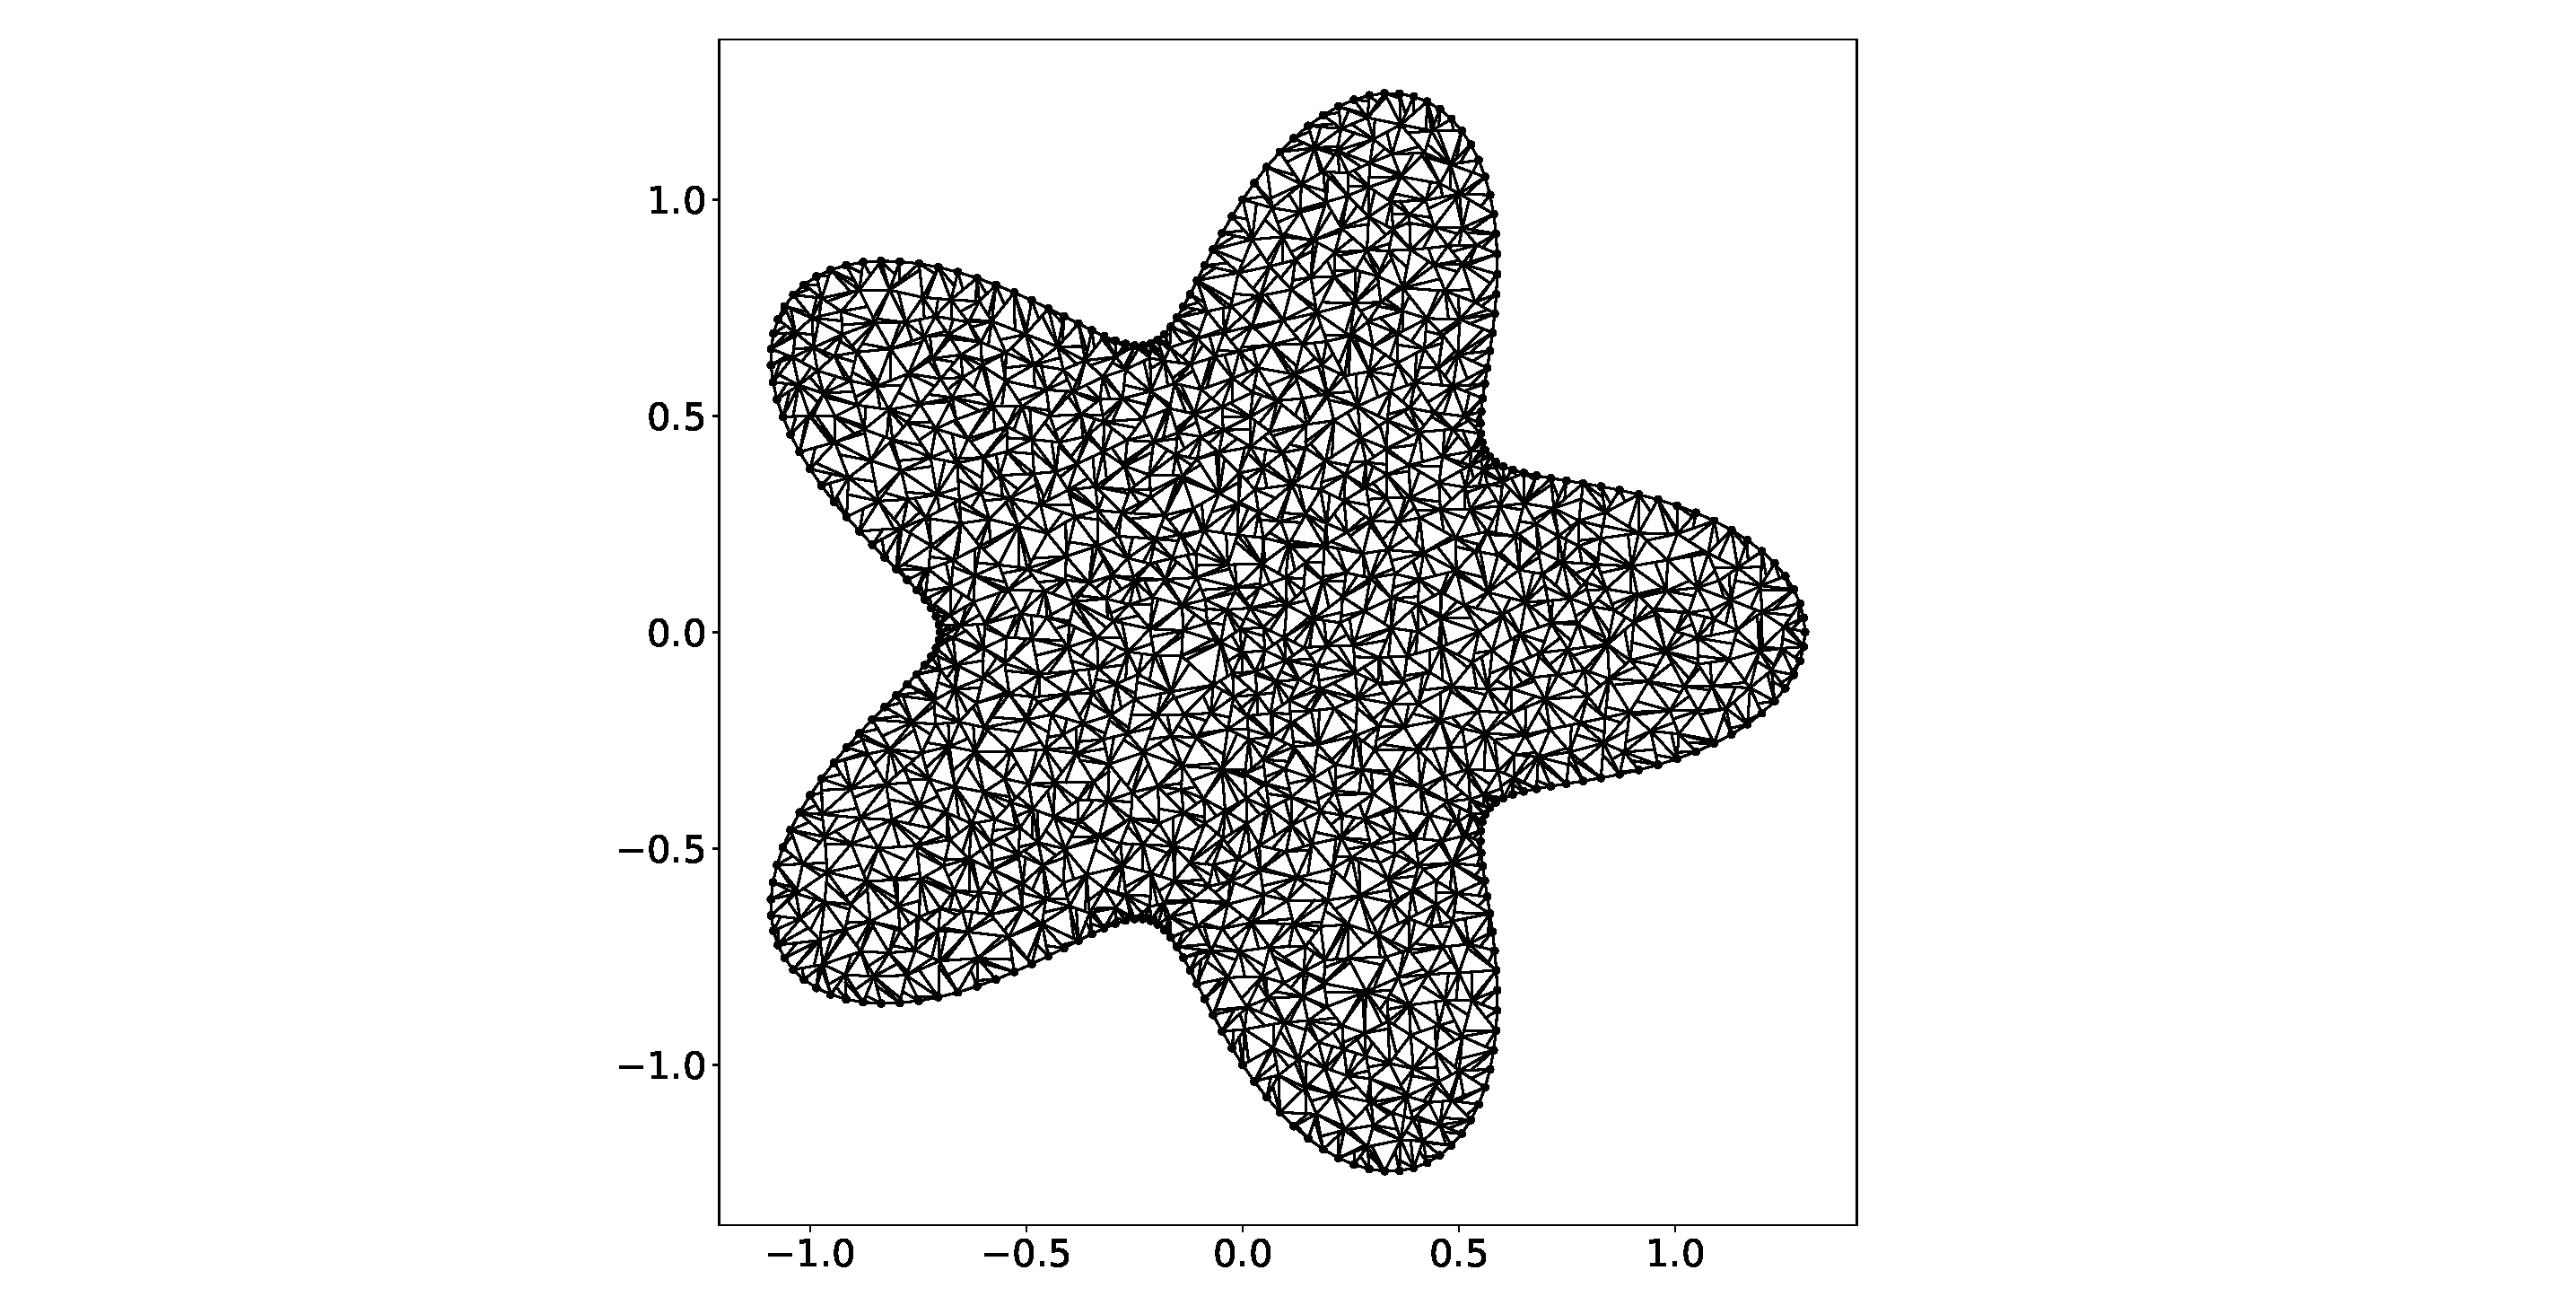
\includegraphics[height=0.66\textheight]{meshdegh1_cropped.pdf}

\vspace{1mm}
\scriptsize
Nonconforming test mesh for $h=0.1$: 127 of the 3624 added triangles are
degenerate.
\end{frame}

% 58
\begin{frame}{Robustness under degraded meshes}
\centering
\resizebox{!}{0.58\textheight}{% This file was created by matlab2tikz.
%
%The latest updates can be retrieved from
%  http://www.mathworks.com/matlabcentral/fileexchange/22022-matlab2tikz-matlab2tikz
%where you can also make suggestions and rate matlab2tikz.
%
\definecolor{mycolor1}{rgb}{0.00000,0.44700,0.74100}%
\definecolor{mycolor2}{rgb}{0.85000,0.32500,0.09800}%
%
\begin{tikzpicture}[scale=0.78]

\begin{axis}[%
%width=4.602in,
%height=3.743in,
%at={(0.772in,0.593in)},
scale only axis,
xmode=log,
xmin=1e-6,
xmax=0.003,
xminorticks=true,
xlabel style={font=\Large\color{white!15!black}},
xlabel={$\delta$},
extra x ticks={0.002},
extra x tick labels={},
xticklabel style = {font=\large},
ymode=log,
ymin=1e-08,
ymax=0.003,
yminorticks=true,
ylabel style={font=\Large\color{white!15!black}},
ylabel={Relative error},
yticklabel style = {font=\large},
axis background/.style={fill=white},
xmajorgrids,
xminorgrids,
ymajorgrids,
yminorgrids,
legend style={font=\Large,at={(0.03,0.97)}, anchor=north west, legend cell align=left, align=left, draw=white!15!black},
clip mode=individual,
]
%%%%%%%%%%%%%%%% non-degenerate %%%%%%%%%%%%%%%%
\addplot [color=mycolor1, line width=1.0pt, mark=*, mark options={solid, mycolor1}, mark size=2.0pt]
  table[row sep=crcr]{%
     9.060379704474429e-04     5.751918073542443e-05\\
     5.228085044004151e-04     2.837455721621307e-05\\
     2.347745798855494e-04     9.370096943038349e-06\\
     6.011487245790398e-05     1.583517743727053e-06\\
     9.710857461079579e-06     8.639670272700639e-07\\
     5.476650070427052e-06     8.177329070598145e-07\\
     2.439060356200125e-06     1.074911344509009e-06\\
};
%\addlegendentry{$e_{\infty}$}

\addplot [color=mycolor2, dotted, line width=1.0pt, mark=o, mark options={solid, mycolor2}, mark size=2.0pt]
  table[row sep=crcr]{%
     9.060379704474429e-04     1.056229717482648e-05\\
     5.228085044004151e-04     4.308129059030584e-06\\
     2.347745798855494e-04     1.289057084765961e-06\\
     6.011487245790398e-05     4.727182728941369e-07\\
     9.710857461079579e-06     9.871963679464511e-08\\
     5.476650070427052e-06     9.626944932492544e-08\\
     2.439060356200125e-06     9.465263375682426e-08\\
};
%\addlegendentry{$e_{2}$}
%%%%%%%%%%%%%%%% degenerate %%%%%%%%%%%%%%%%
\addplot [color=mycolor1, line width=1.0pt, mark=square*, mark options={solid, mycolor1}, mark size=2.0pt]
  table[row sep=crcr]{%
     9.060379704474449e-04     7.973889932925468e-05\\
     5.228085044004164e-04     3.634742411910547e-05\\
     2.347745798855498e-04     1.150546410135194e-05\\
     6.011487245790397e-05     1.571959278818947e-06\\
     9.710857461079581e-06     1.081793863973289e-06\\
     5.476650070427052e-06     1.079304478629404e-06\\
     2.439060356200125e-06     1.070292899523101e-06\\
};
%\addlegendentry{$e_{\infty}^{*}$}

\addplot [color=mycolor2, dotted, line width=1.0pt, mark=square, mark options={solid, mycolor2}, mark size=2.0pt]
  table[row sep=crcr]{%
     9.060379704474449e-04     1.066619380494925e-05\\
     5.228085044004164e-04     4.307149939723041e-06\\
     2.347745798855498e-04     1.287671339463834e-06\\
     6.011487245790397e-05     4.771734810266285e-07\\
     9.710857461079581e-06     9.840691074091229e-08\\
     5.476650070427052e-06     9.593914360271627e-08\\
     2.439060356200125e-06     9.456357000868728e-08\\
};
%\addlegendentry{$e_{2}^{*}$}
%%%%%%%%%%%% reference lines %%%%%%%%%%%%%%%%%

\addplot [color=black, dashed, line width=1.0pt]
  table[row sep=crcr]{%
     9.060379704474450e-04     1.720452232222099e-04\\
     5.228085044004167e-04     7.541139705766146e-05\\
     2.347745798855497e-04     2.269340319540672e-05\\
     6.011487245790398e-05     2.940328925231237e-06\\
   };

\addplot [color=black, dashed, line width=1.0pt]
  table[row sep=crcr]{%
     9.060379704474450e-04     1.720452232222099e-05\\
     5.228085044004167e-04     7.541139705766145e-06\\
     2.347745798855497e-04     2.269340319540672e-06\\
%     6.011487245790398e-05     2.940328925231237e-07\\
};
%\addlegendentry{$O(\delta^{(3/2})$}
\end{axis}


\end{tikzpicture}%
%%% Local Variables:
%%% mode: latex
%%% TeX-master: ../poissongaussfryk.tex
%%% End:
}

\vspace{1mm}
\scriptsize
Round and square markers denote the conforming and degraded mesh sequences,
respectively; solid and dotted curves are relative $\ell_\infty$ and $\ell_2$
errors. The reported test also includes high-aspect-ratio elements and small gaps.
\end{frame}

% 56
\begin{frame}{Poisson-NUFFT summary}
\small
\begin{enumerate}
  \item The volume potential is represented as a heat potential.
  \item Short time is local and handled by asymptotics plus dyadic correction.
  \item Near and far history are smooth Fourier integrals.
  \item The NUFFT handles nonuniform source and target locations.
  \item Boundary data are imposed by a standard BIE correction.
  \item The geometry interface consists of quadrature nodes, weights, normals,
  and target points.
\end{enumerate}
\end{frame}

% 57
\begin{frame}{Break}
\centering
\Large
10 minute break

\vspace{6mm}
\normalsize
After the break: recursive reduction quadrature for 3D layer potentials.
\end{frame}

\section{Recursive Reduction Quadrature}

% 58
\begin{frame}{RRQ objectives}
\small
The main mathematical and algorithmic objectives are:
\begin{enumerate}
  \item identify the self, near, and close target regimes in 3D;
  \item explain why close evaluation has no natural target-centered surface
  parameterization;
  \item state the RRQ reduction chain;
  \item explain the role of harmonic polynomial density approximation;
  \item use Stokes theorem to understand surface-to-line reduction;
  \item describe why singularity-swap quadrature removes adaptive line integration.
\end{enumerate}
\end{frame}

% 59
\begin{frame}{3D Laplace layer potentials}
\small
For a smooth surface $S\subset\R^3$,
\[
  \Sop[\sigma](\rp)
  =
  \int_S G(\rp,\rvec)\sigma(\rvec)\dd a(\rvec),
\]
\[
  \Dop[\mu](\rp)
  =
  \int_S
  \frac{\partial G(\rp,\rvec)}{\partial \nu_{\rvec}}
  \mu(\rvec)\dd a(\rvec),
\]
where
\[
  G(\rp,\rvec)=\frac{1}{4\pi|\rp-\rvec|}.
\]
Here $\rp$ is the target, $\rvec$ is the source, and
$\partial/\partial\nu_{\rvec}$ denotes differentiation in the outward source
normal direction at $\rvec\in S$.
\end{frame}

% 60
\begin{frame}{Normal derivatives}
\small
RRQ also treats
\[
  \Spop[\sigma](\rp)
  =
  \int_S
  \frac{\partial G(\rp,\rvec)}{\partial \nu_{\rp}}
  \sigma(\rvec)\dd a(\rvec),
\]
and
\[
  \Dpop[\mu](\rp)
  =
  \int_S
  \frac{\partial^2G(\rp,\rvec)}
       {\partial\nu_{\rp}\partial\nu_{\rvec}}
  \mu(\rvec)\dd a(\rvec).
\]

\begin{block}{Quadrature issue}
The kernels range from weakly singular to hypersingular. Near the surface,
ordinary smooth quadrature deteriorates rapidly.
\end{block}
\[
  \nu_{\rp}\text{ is the target normal for }\rp\in S,\qquad
  \nu_{\rvec}\text{ is the source normal.}
\]
\end{frame}

% 61
\begin{frame}{Four target regimes}
\small
For one source patch $P$:
\begin{enumerate}
  \item \textbf{Smooth interaction}: target is sufficiently far from $P$.
  \item \textbf{Self interaction}: target is on $P$.
  \item \textbf{Near interaction}: target is on $S$ and close to $P$.
  \item \textbf{Close evaluation}: target is off surface and close to $P$.
\end{enumerate}

\begin{block}{Most difficult case}
Close evaluation is the most delicate regime because the target has no natural
parameter value on the source patch.
\end{block}
\end{frame}

% 62
\begin{frame}{Self-interaction on the source patch}
\small
When the target lies on the source patch:
\begin{itemize}
  \item local coordinates can be centered at the target;
  \item singularity subtraction or polar/Duffy transformations are natural;
  \item the parameter-space location of the singularity is known.
\end{itemize}

When the target is close but off the surface:
\begin{itemize}
  \item the closest point may not be well behaved near patch edges;
  \item singularity cancellation in parameter space is less direct;
  \item interpolation/extrapolation can become delicate.
\end{itemize}
\end{frame}

% 63
\begin{frame}{Matrix split in a fast BIE solver}
\small
For a discretized layer potential matrix,
\[
  \bm D=\bm D_{\rm smooth}+\bm D_{\rm RRQ}.
\]

\begin{itemize}
  \item $\bm D_{\rm smooth}$ uses source-dependent smooth quadrature weights.
  \item At fixed precision, the FMM applies $\bm D_{\rm smooth}$ in
  $\cO(N_S)$ work for $N_S$ source nodes.
  \item $\bm D_{\rm RRQ}$ corrects self, near, and close interactions.
  \item For typical geometries, only $\cO(1)$ targets are close to one patch;
  $\bm D_{\rm RRQ}$ is therefore sparse.
\end{itemize}
\end{frame}

% 64
\begin{frame}{RRQ reduction chain}
\small
\[
  \boxed{
  \text{surface integral}
  \longrightarrow
  \text{line integral}
  \longrightarrow
  \text{analytic 1D recurrences}
  }
\]

\begin{block}{Reason for the term recursive}
The first reduction uses Stokes theorem on the surface patch. The second
reduction uses a complex-parameter integration-by-parts identity along the boundary
curve.
\end{block}
\end{frame}

% 65
\begin{frame}{Patch-level problem}
\small
Focus on one smooth triangular patch $P$.
\[
  \Dop[\mu](\rp)
  =
  \int_P
  \nabla_{\rvec} G(\rp,\rvec)\cdot\nuvec(\rvec)
  \mu(\rvec)\dd a(\rvec).
\]

Assume:
\begin{itemize}
  \item $P$ is smooth and contractible;
  \item the density is smooth on $P$;
  \item $P$ has high-order geometry nodes;
  \item target $\rp$ may be on, near, or close to $P$.
\end{itemize}
\end{frame}

% 66
\begin{frame}{Patch normalization}
\small
Before forming local approximation systems:
\begin{itemize}
  \item translate the patch so the mean of the three vertices is at the origin;
  \item rotate so the three vertices lie on the $xy$-plane;
  \item scale so the longest side length is one.
\end{itemize}

\begin{block}{Purpose}
This makes the basis and conditioning less sensitive to mesh scale and
separates shape/curvature effects from simple size effects.
\end{block}
\end{frame}

% 67
\begin{frame}{Approximation target for RRQ}
\small
The density is approximated by harmonic polynomial data that extend naturally
off the surface.

Here $H^{(l,m)}$ are real regular harmonic polynomials of degree $l$.

For the double layer, RRQ uses a quaternion harmonic approximation:
\[
  (\mu(\rvec),\bm 0)
  \approx
  \sum_{l=1}^p\sum_{m=1}^l
  (0,\nabla H^{(l,m)}(\rvec))\,c^{(l,m)}.
\]

\end{frame}

% 68
\begin{frame}{Quaternion algebra}
\small
Write a quaternion as $q=(q_0,\bm q)$ with scalar part $q_0$ and vector part
$\bm q\in\R^3$.

The product is
\[
  (f_0,\bm f)(g_0,\bm g)
  =
  (f_0g_0-\bm f\cdot\bm g,\,
   f_0\bm g+g_0\bm f+\bm f\times\bm g).
\]

\begin{itemize}
  \item Dot products and cross products appear automatically.
  \item Multiplication is associative but not commutative.
  \item The scalar part extracts the physical layer potential.
\end{itemize}
\end{frame}

% 69
\begin{frame}{Quaternion parametrization of rotated patches}
\small
For the DLP,
\[
  (0,\nabla G)(0,\nuvec)(\mu,\bm0)
  =
  \left(
  -(\nabla G\cdot\nuvec)\mu,\,
  (\nabla G\times\nuvec)\mu
  \right).
\]

Thus
\[
  \Dop[\mu](\rp)=-Q_0[\mu](\rp),
\]
where $Q_0$ is the scalar part of the corresponding quaternion integral.

\begin{block}{Role of quaternion notation}
The quaternion notation packages the scalar potential and auxiliary vector
forms in one algebraic object.
\end{block}
\end{frame}

% 70
\begin{frame}{General Stokes theorem}
\small
For a differential form $\omega$ on an oriented patch $P$,
\[
  \int_{\partial P}\omega=\int_P d\omega.
\]

If a 2-form $\alpha$ is closed,
\[
  d\alpha=0,
\]
and the patch is contractible, then by the Poincare lemma it is exact:
\[
  \alpha=d\beta.
\]
Therefore
\[
  \int_P \alpha=\int_{\partial P}\beta.
\]
\end{frame}

% 71
\begin{frame}{Deriving the vector area differential}
\small
Let an oriented patch be parametrized by
\[
  \rvec(\theta,\phi)=(x(\theta,\phi),y(\theta,\phi),z(\theta,\phi)).
\]
Then standard vector calculus gives
\[
  \nuvec(\rvec)\dd a(\rvec)
  =\left(\frac{\partial\rvec}{\partial\theta}
  \times\frac{\partial\rvec}{\partial\phi}\right)
  d\theta\wedge d\phi.
\]
For its first component,
\[
\begin{aligned}
  dy\wedge dz
  &=(y_\theta d\theta+y_\phi d\phi)
    \wedge(z_\theta d\theta+z_\phi d\phi)\\
  &=(y_\theta z_\phi-y_\phi z_\theta)\,d\theta\wedge d\phi
   =\left(\rvec_\theta\times\rvec_\phi\right)_1
     d\theta\wedge d\phi.
\end{aligned}
\]
The cyclic identities for $dz\wedge dx$ and $dx\wedge dy$ give the other
two components.
\end{frame}

% 72
\begin{frame}{Surface integrals as 2-forms}
\small
The vector area differential is
\[
  \nuvec(\rvec)\dd a(\rvec)
  =
  dy\wedge dz\,\mathbf i
  +dz\wedge dx\,\mathbf j
  +dx\wedge dy\,\mathbf k.
\]

Thus
\[
  \int_S \bm f(\rvec)\cdot\nuvec(\rvec)\dd a(\rvec)
  =
  \int_S f_1\,dy\wedge dz
  +f_2\,dz\wedge dx
  +f_3\,dx\wedge dy.
\]
\end{frame}

% 73
\begin{frame}{DLP quaternion 2-form}
\small
For $\rvec\ne\rp$, set
\[
  \bm g(\rvec)=\nabla_{\rvec}G(\rp,\rvec),
  \qquad
  \bm f(\rvec)=\nabla H^{(l,m)}(\rvec).
\]
Both are gradients of harmonic functions. Using the vector area differential,
the DLP basis integrand is the quaternion-valued 2-form
\[
  \alpha_D^{(l,m)}(\rp,\rvec)
  =(0,\bm g(\rvec))(0,\nuvec(\rvec))(0,\bm f(\rvec))\dd a(\rvec).
\]
The next slide verifies its closedness component by component.
\end{frame}

% 74
\begin{frame}{Divergence-free fields give exact 2-forms}
\small
For a target $\rp\notin P$, choose a contractible neighborhood $U\supset P$
that does not contain $\rp$. For a smooth vector field $\bm F$ on $U$, define
\[
  \omega_{\bm F}
  =F_1\,\dd y\wedge\dd z+F_2\,\dd z\wedge\dd x+F_3\,\dd x\wedge\dd y.
\]
Its restriction to $P$ is the vector-area integrand, and its exterior derivative is
\[
  \omega_{\bm F}|_P=(\bm F\cdot\nuvec)\dd a,
  \qquad
  \dd\omega_{\bm F}=(\nabla\cdot\bm F)\dd x\wedge\dd y\wedge\dd z.
\]
Hence $\nabla\cdot\bm F=0$ makes $\omega_{\bm F}$ closed on $U$.
The Poincar\'{e} lemma on the contractible set $U$ then gives a 1-form
$\eta_{\bm F}$ with $\omega_{\bm F}=\dd\eta_{\bm F}$. Restricting to $P$,
\[
  \int_P \bm F\cdot\nuvec\,\dd a
  =\int_P \dd\eta_{\bm F}
  =\int_{\partial P}\eta_{\bm F}.
\]

\footnotesize M. P. do Carmo, \emph{Differential Forms and Applications}, Springer, 1998.
\end{frame}

\begin{frame}{The DLP components are divergence-free}
\small
Write $\bm g=\nabla\psi$ and $\bm f=\nabla\phi$, where
$\Delta\psi=\Delta\phi=0$ on $U$. Quaternion multiplication gives
\[
  (0,\bm g)(0,\nuvec)(0,\bm f)
  =\left(-\left(\bm g\times\nuvec\right)\cdot\bm f,\,
  -\left(\bm g\cdot\nuvec\right)\bm f
  +\left(\bm g\times\nuvec\right)\times\bm f\right).
\]
Thus its scalar component is $\bm F_0\cdot\nuvec\,\dd a$, with
\[
  \bm F_0=-\bm f\times\bm g,
  \qquad \nabla\cdot\bm F_0=0,
\]
and its $i$th vector component is $\bm F_i\cdot\nuvec\,\dd a$, with
\[
  \bm F_i=(\bm g\cdot\bm f)\mathbf e_i-g_i\bm f-f_i\bm g,
  \qquad i=1,2,3.
\]
Indeed,
\[
  \nabla\cdot\bm F_i
  =\partial_i(\bm g\cdot\bm f)-\nabla g_i\cdot\bm f-g_i\Delta\phi
   -\nabla f_i\cdot\bm g-f_i\Delta\psi=0.
\]
The first term cancels the two gradient terms, and the remaining Laplacians
vanish. By the preceding slide, all four components are exact; hence
$\dd\beta_D^{(l,m)}=\alpha_D^{(l,m)}$.

\footnotesize H. Zhu and S. Veerapaneni, \emph{SIAM J. Sci. Comput.} 44(3):A1381--A1404, 2022, Lemma 3.3 and Corollary 3.4.
\end{frame}

% 75
\begin{frame}{DLP reduction to line integrals}
\small
With the quaternion density approximation,
\[
  (\mu(\rvec),\bm0)
  \approx\sum_{l=1}^p\sum_{m=1}^l
  (0,\nabla H^{(l,m)}(\rvec))c^{(l,m)},
\]
the double-layer potential satisfies
\[
\begin{aligned}
  \Dop[\mu](\rp)
  &\approx-\sum_{l,m}\int_P
    \left[\alpha_D^{(l,m)}(\rp,\rvec)c^{(l,m)}\right]_0\\
  &=-\sum_{l,m}\int_{\partial P}
    \left[\beta_D^{(l,m)}(\rp,\rvec)c^{(l,m)}\right]_0.
\end{aligned}
\]
Here $[\cdot]_0$ denotes the scalar part of a quaternion.  The density fit is
the only approximation in this reduction; Stokes' theorem itself is exact.
\end{frame}

% 75
\begin{frame}{Harmonic polynomials}
\small
Regular solid harmonics are
\[
  R_l^m(\rvec)
  =
  \frac{1}{\sqrt{2l+1}}r^lY_l^m(\theta,\phi).
\]
Here $(r,\theta,\phi)$ are spherical polar coordinates of $\rvec$ and
$Y_l^m$ is a spherical harmonic.  The $R_l^m$ are homogeneous harmonic
polynomials of degree $l$.

RRQ uses rotated real combinations
\[
  H^{(l,m)}(x,y,z)=\widetilde H^{(l,m)}(y,z,x).
\]

\end{frame}

% 76
\begin{frame}{Basis completeness on a flat triangle}
\small
For the chosen basis,
\[
  \nabla H^{(l,m)}(x,y,0)
  =
  (0,0,F^{(l,m)}(x,y)).
\]
For any order $p$,
\[
  \Span\{F^{(l,m)}:1\le m\le l\le p\}
  =
  \Span\{x^iy^j:0\le i+j\le p-1\}.
\]

\begin{block}{Consequence}
The harmonic approximation has the same polynomial approximation power as
standard order-$p$ interpolation on a flat triangle.
\end{block}
\end{frame}

% 77
\begin{frame}{Collocation system for the DLP density}
\small
At the $n_p=p(p+1)/2$ collocation nodes $\rvec^{(i,j)}$ on $P$
($0\le i+j\le p-1$), solve
\[
  \sum_{l=1}^p\sum_{m=1}^l
  (0,\nabla H^{(l,m)}(\rvec^{(i,j)}))c^{(l,m)}
  =
  (\mu(\rvec^{(i,j)}),\bm0).
\]

The full system has size
\[
  4n_p\times 4n_p.
\]
\end{frame}

% 78
\begin{frame}{Block form of the quaternion system}
\small
Let $F_1,F_2,F_3\in\R^{n_p\times n_p}$ collect the three components of
$\nabla H^{(l,m)}$ at the collocation nodes.  If
$\bm c_q\in\R^{n_p}$ collects the $q$th quaternion coefficient component,
then
\[
\begin{pmatrix}
  0 & -F_1 & -F_2 & -F_3\\
  F_1 & 0 & -F_3 & F_2\\
  F_2 & F_3 & 0 & -F_1\\
  F_3 & -F_2 & F_1 & 0
\end{pmatrix}
\begin{pmatrix}\bm c_0\\\bm c_1\\\bm c_2\\\bm c_3\end{pmatrix}
=
\begin{pmatrix}\bm\mu\\\bm0\\\bm0\\\bm0\end{pmatrix}.
\]

On a flat patch, only the $F_3$ block remains. Invertibility reduces to the
usual invertibility of polynomial interpolation at the chosen nodes.
\end{frame}

% 80
\begin{frame}{The SLP 2-form}
\small
The SLP integrand is
\[
  G(\rp,\rvec)\sigma(\rvec)\dd a(\rvec),
\]
which is not directly a quaternion DLP 2-form.

For $v=H^{(l,m)}$ and $\rvec\ne\rp$, define
\[
  \chi^{(l,m)}(\rp,\rvec)
  =\bigl(G(\rp,\rvec)\nabla H^{(l,m)}(\rvec)
   -H^{(l,m)}(\rvec)\nabla G(\rp,\rvec)\bigr)
   \cdot\nuvec(\rvec)\dd a(\rvec).
\]
Because $G(\rp,\cdot)$ and $H^{(l,m)}$ are harmonic away from $\rp$,
\[
  d\chi^{(l,m)}
  =\bigl(G\Delta H^{(l,m)}-H^{(l,m)}\Delta G\bigr)
    \,dx\wedge dy\wedge dz=0.
\]
Thus $\chi^{(l,m)}$ is closed and exact on a contractible patch.
\end{frame}

% 81
\begin{frame}{SLP reduction theorem}
\small
Approximate the SLP density by
\[
  \sigma(\rvec)
  \approx
  \sum_{l=1}^p\sum_{m=1}^l
  \nabla H^{(l,m)}(\rvec)\cdot\nuvec(\rvec)\,d^{(l,m)}.
\]
Define an intermediate density
\[
  \rho(\rvec)=\sum_{l,m}H^{(l,m)}(\rvec)d^{(l,m)}.
\]

Then the SLP is reduced to a combination of SLP-type 1-forms and DLP-type
1-forms for $\rho$.
\end{frame}

% 82
\begin{frame}{Target-centered 1-forms}
\small
The 1-form primitive is not unique. Older origin-centered forms lose translation
invariance of the singularity.

RRQ chooses the reference point
\[
  \bm p=\rp.
\]

\begin{block}{Effect}
The resulting line integrals have kernels with singularity structure depending
on $\rvec-\rp$, like the original Green's function.
\end{block}
\[
  \text{same singularity}
  \quad\Longrightarrow\quad
  \text{singularity-swap quadrature applies.}
\]
\end{frame}

% 83
\begin{frame}{Cost of origin-centered differential forms}
\small
If the 1-form is built around a fixed origin, the line-integral kernel depends on
absolute source and target coordinates.

\begin{itemize}
  \item Translation invariance is lost.
  \item The near singularity is weaker but more complicated.
  \item Adaptive integration may be required along patch edges.
\end{itemize}

\begin{block}{RRQ improvement}
Use target-centered forms, then evaluate nearly singular line integrals by
analytic recurrences rather than adaptive integration.
\end{block}
\end{frame}

% 84
\begin{frame}{Singularity-preserving line integrals}
\small
After reduction, the line integral on a patch edge has the schematic form
\[
  \int_{\partial P}
  \frac{\text{smooth polynomial/geometric data}}
       {|\rvec(t)-\rp|^m}\dd t,
  \qquad m=1,3,\ldots.
\]

\begin{itemize}
  \item The dimension is now one.
  \item The line integrand retains the target-dependent kernel factor
  $1/|\rvec(t)-\rp|^m$.
  \item The next step factors the analytically continued squared distance using
  complex roots in the edge parameter.
\end{itemize}
\end{frame}

% 85
\begin{frame}{Singularity-swap quadrature}
\small
Consider a nearly singular line integral
\[
  I(\rp)=\int_{-1}^1
  \frac{f(t)}{|\rvec(t)-\rp|^m}\dd t.
\]
Find a complex number $t_0$ such that
\[
  (x(t_0)-x')^2
  +(y(t_0)-y')^2
  +(z(t_0)-z')^2
  =
  0.
\]

\begin{block}{Meaning}
The closest complex singularity is expressed in the parameter plane, not in
physical space.
\end{block}
\end{frame}

% 86
\begin{frame}{The swap}
\small
Rewrite
\[
  I(\rp)
  =
  \int_{-1}^1
  \frac{F(t)}
       {((t-t_0)(t-\overline{t_0}))^{m/2}}
  \dd t,
\]
where
\[
  F(t)
  =
  f(t)
  \frac{|t-t_0|^m}{|\rvec(t)-\rp|^m}.
\]

\begin{itemize}
  \item $F(t)$ is smooth on $[-1,1]$.
  \item The singular dependence is isolated in known moments.
  \item The singularity-swap construction evaluates the resulting moments
  analytically.
\end{itemize}
\end{frame}

% 87
\begin{frame}{Moment recurrences}
\small
After approximating $F$ by a polynomial,
\[
  F(t)\approx\sum_{i=0}^{q}a_i t^i,
\]
the required building blocks are
\[
  I_i(t_0)
  =
  \int_{-1}^1
  \frac{t^i}
       {((t-t_0)(t-\overline{t_0}))^{m/2}}
  \dd t.
\]
The singularity-swap construction evaluates these moments by recurrence.
\end{frame}

% 89
\begin{frame}{The second reduction}
\small
The first reduction:
\[
  \int_P \text{2-form}
  =
  \int_{\partial P}\text{1-form}.
\]

The second reduction:
\[
  \int_{\partial P}\text{singularity-preserving 1D kernel}
  =
  \text{weighted sum of analytic moments}.
\]

\begin{block}{Recursive reduction}
The surface integral is recursively reduced until the remaining singular
behavior is captured by explicit one-dimensional formulas.
\end{block}
\end{frame}

% 89
\begin{frame}{RRQ pipeline}
\centering
\begin{tikzpicture}[
  scale=0.96,
  transform shape,
  node distance=1.4cm,
  box/.style={draw,rounded corners=1mm,align=center,minimum width=2.6cm,minimum height=0.8cm},
  arr/.style={-{Latex[length=2mm]},thick}
]
\node[box,fill=CCMorange!20] (patch) {patch $P$\\density samples};
\node[box,fill=black!5,right=of patch] (harm) {harmonic\\approximation};
\node[box,fill=black!5,right=of harm] (stokes) {Stokes\\surface to line};
\node[box,fill=black!5,right=of stokes] (swap) {singularity\\swap};
\node[box,fill=SFdark!10,below=of stokes] (value) {corrected\\potential value};
\draw[arr] (patch) -- (harm);
\draw[arr] (harm) -- (stokes);
\draw[arr] (stokes) -- (swap);
\draw[arr] (swap) |- (value);
\end{tikzpicture}
\end{frame}

% 90
\begin{frame}{Algorithm: source-dependent setup}
\small
For a fixed patch and order $p$:
\begin{enumerate}
  \item evaluate $S_l^m(\rvec^{(i,j)})$ and gradients at patch collocation nodes;
  \item construct the quaternion density system;
  \item solve for coefficients $c^{(l,m)}$;
  \item evaluate the basis and gradients at interpolation nodes on $\partial P$.
\end{enumerate}

\begin{block}{Cost}
Matrix construction costs $\cO(p^4)$ and the dense local solve costs
$\cO(p^6)$ per patch.
\end{block}
\end{frame}

% 91
\begin{frame}{Algorithm: target-dependent setup}
\small
For a target $\rp$:
\begin{enumerate}
  \item evaluate $S_l^m(\rp)$ and gradients;
  \item form the target-centered singularity-preserving line integrals;
  \item evaluate the singularity-swap moments;
  \item assemble line integrals for all $(l,m)$.
\end{enumerate}

\begin{block}{Cost}
The target-dependent line-integral work is $\cO(p^3)$ per target-patch
special interaction.
\end{block}
\end{frame}

% 92
% 93
\begin{frame}{Source and target cost summary}
\small
Let $N_S$ be the total number of source points and $N_T$ the number of target
points requiring special quadrature.

\[
  \text{patch setup cost}\sim \cO(N_Sp^4),
\]
\[
  \text{special target cost}\sim \cO(N_Tp^3).
\]

\begin{block}{Solve phase}
During the BIE solve phase, $N_T$ is typically $2$--$4$ times $N_S$ for
reasonable geometries.
\end{block}
\end{frame}

% 94
\begin{frame}{Other layer potentials}
\small
The same RRQ architecture applies to:
\[
  \Sop,\qquad \Dop,\qquad \partial_\nu\Sop,\qquad \partial_\nu\Dop.
\]

\begin{itemize}
  \item The single layer uses both scalar and quaternion density approximations.
  \item The normal derivative of the single layer is closely analogous to the
  double-layer construction.
  \item The normal derivative of the double layer uses differentiated forms.
\end{itemize}

\begin{block}{Implementation consequence}
Once the 1-form and moment machinery is implemented, the four Laplace operators
share most of the numerical infrastructure.
\end{block}
\end{frame}

% 95
\begin{frame}{Target grouping}
\small
RRQ divides close targets into two groups:
\begin{itemize}
  \item targets close to the surface but sufficiently away from the patch edges;
  \item targets close to the patch edges.
\end{itemize}

\begin{block}{Computational consequence}
For the first group, evaluating the line integrals requires much less work. For
the second group, singularity-swap quadrature requires only a mild increase in work.
\end{block}

\[
  \text{The targets requiring significant work lie near the patch boundary.}
\]
\end{frame}

% 96
\begin{frame}{Curvature raises the local RRQ system condition number}
\small
For a paraboloid patch with side length $h=1$, $H$ denotes the maximum mean
curvature.
\par\smallskip
\centering
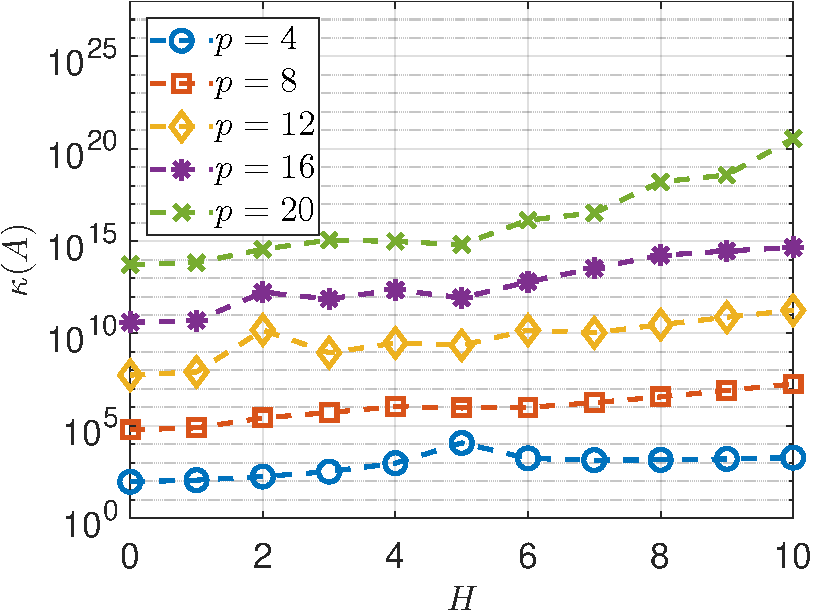
\includegraphics[height=0.48\textheight]{condnum_curv.pdf}
\par\vspace{0.5mm}
\begin{block}{What the plot shows}
At fixed $h$, the condition number $\kappa(A)$ increases with both the maximum
mean curvature $H$ and the approximation order $p$.
\end{block}
\end{frame}

% 97
\begin{frame}{Smaller patches recover flat-patch conditioning}
\small
For the same paraboloid, fix $H=10$ and take the patch side length
$h=2^{-L}$, $L=0,\ldots,10$.
\par\smallskip
\centering
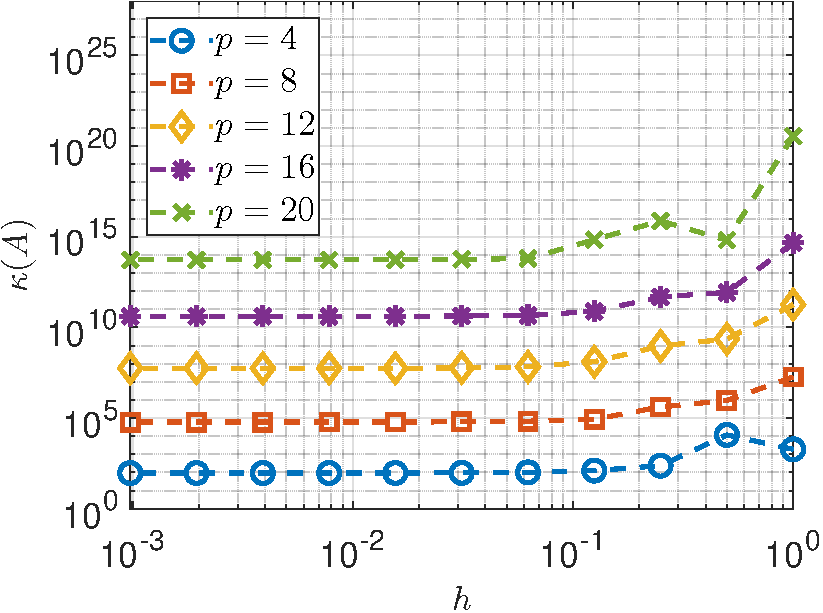
\includegraphics[height=0.48\textheight]{condnum_size.pdf}
\par\vspace{0.5mm}
\begin{block}{What the plot shows}
As $h$ decreases, the patch is better approximated by its tangent plane. A
tenfold reduction in $h$ gives a condition number close to that of a flat patch.
\end{block}
\end{frame}

% 98
\begin{frame}{Harmonic order rapidly increases the condition number}
\small
For a flat equilateral triangle, the local quaternion interpolation matrix $A$
is studied as the approximation order $p$ grows.
\par\smallskip
\centering
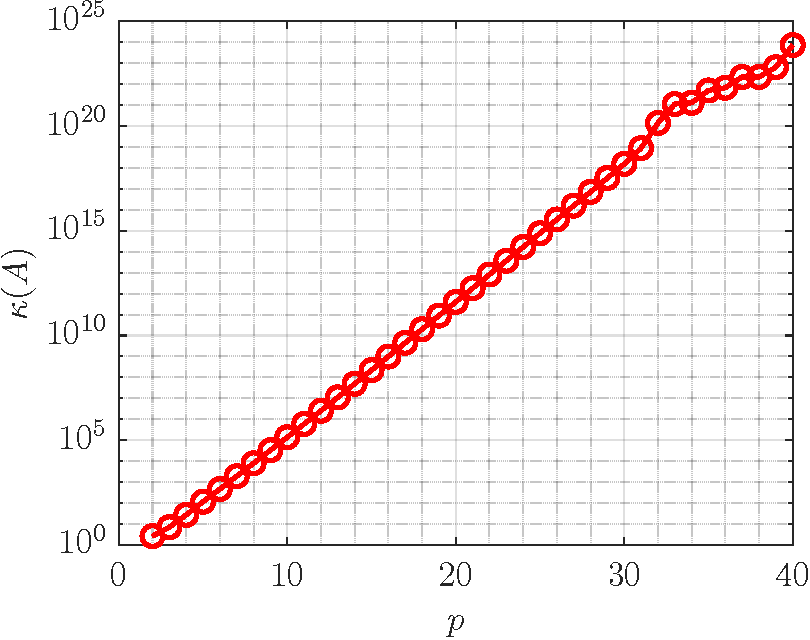
\includegraphics[height=0.48\textheight]{condnum_order.pdf}
\par\vspace{0.5mm}
\begin{block}{Numerical threshold}
In this experiment, $\kappa(A)$ reaches $1/\varepsilon_{\rm mach}$ at $p=26$.
\end{block}
\end{frame}

% 99
\begin{frame}{Coefficient size estimates attainable interpolation accuracy}
\small
For $\mu(x,y)=1/(x^2+y^2+0.5)$ on a flat equilateral triangle, compare the
estimated interpolation error with $\varepsilon_{\rm mach}\|c\|_2$.
\par\smallskip
\centering
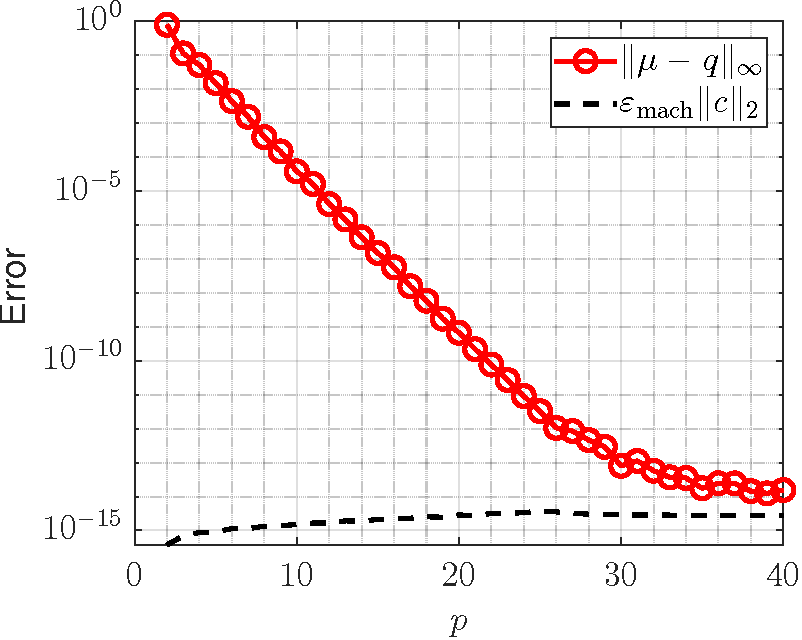
\includegraphics[height=0.48\textheight]{interp_error.pdf}
\par\vspace{0.5mm}
\begin{block}{What the plot shows}
$\varepsilon_{\rm mach}\|c\|_2$ gives an excellent estimate of the highest
attainable accuracy. Here the interpolation error continues to decrease beyond $p=26$.
\end{block}
\end{frame}

% 100
\begin{frame}{Unit sphere: Green's formula follows the expected $O(h^p)$ rates}
\small
\begin{columns}[T,totalwidth=\textwidth]
\begin{column}{0.49\textwidth}
\centering
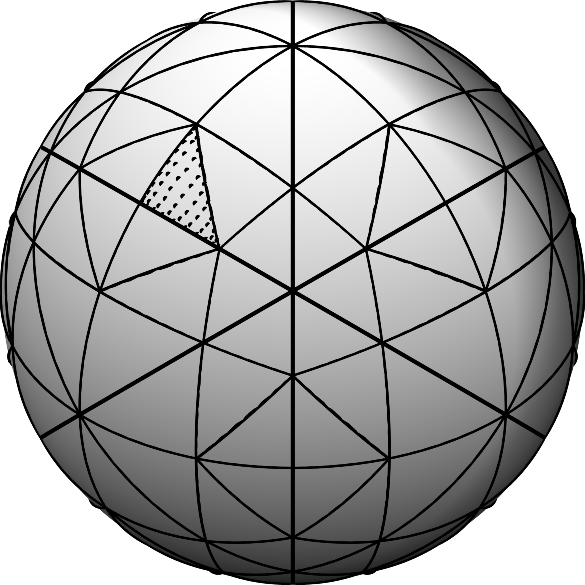
\includegraphics[width=\textwidth,height=0.44\textheight,keepaspectratio]{sphere_geo.pdf}
\par\footnotesize Triangulated unit sphere.
\end{column}
\begin{column}{0.47\textwidth}
\centering
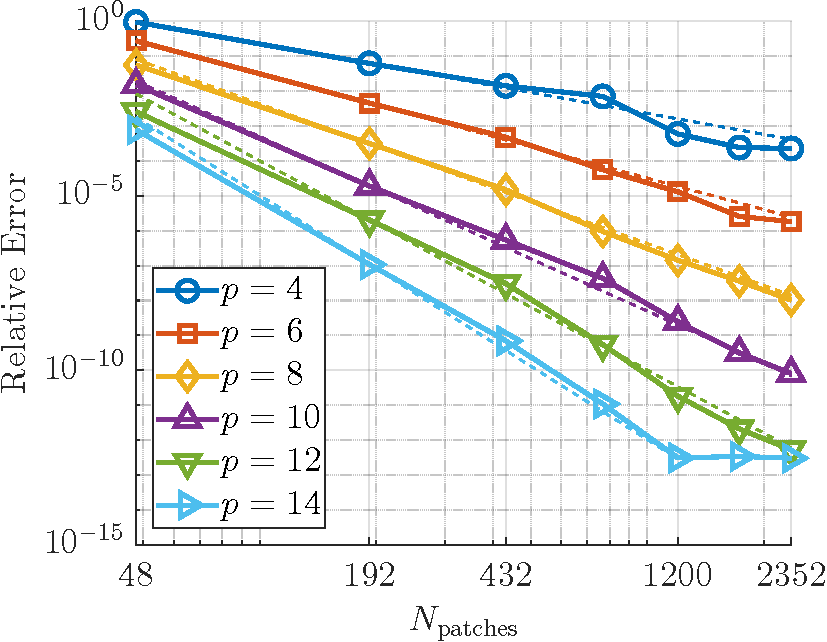
\includegraphics[width=\textwidth,height=0.50\textheight,keepaspectratio]{sphere_convergence_GRF_v3.pdf}
\par\footnotesize Relative $\ell_\infty$ error versus $N_{\rm patches}$.
\end{column}
\end{columns}
\vspace{0.5mm}
\begin{block}{Interpretation}
$N_{\rm patches}=12n^2$ and $h=1/n$; dashed lines show the expected $O(h^p)$
rates. Exact smooth geometry and a test without a BIE solve give clear order separation.
\end{block}
\end{frame}

% 99
\begin{frame}{Warped torus: relative errors under mesh refinement}
\small
\begin{columns}[T,totalwidth=\textwidth]
\begin{column}{0.49\textwidth}
\centering
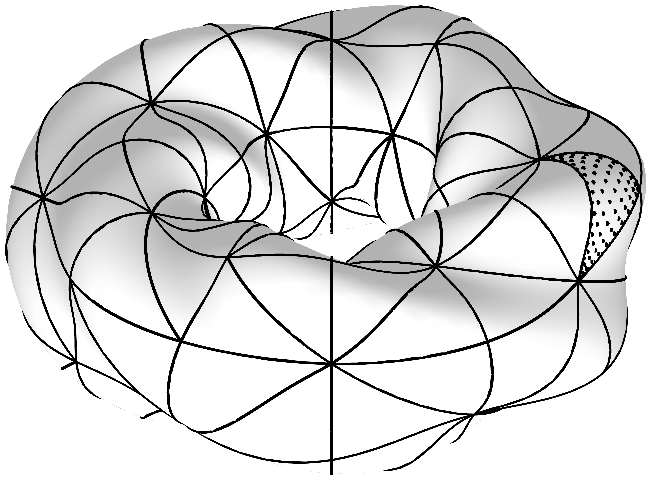
\includegraphics[width=\textwidth,height=0.44\textheight,keepaspectratio]{torus_geo3.pdf}
\par\footnotesize Triangulated warped torus.
\end{column}
\begin{column}{0.47\textwidth}
\centering
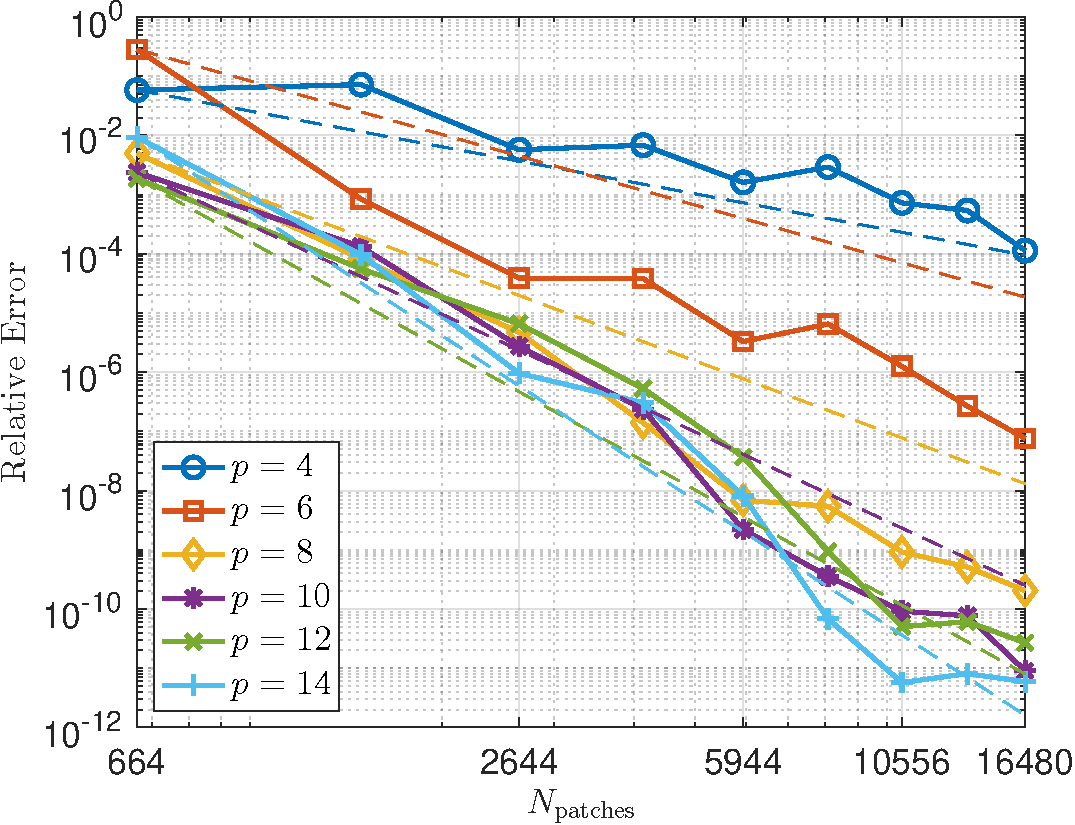
\includegraphics[width=\textwidth,height=0.50\textheight,keepaspectratio]{torus_convergence.pdf}
\par\footnotesize Relative $\ell_\infty$ error versus $N_{\rm patches}$.
\end{column}
\end{columns}
\vspace{0.5mm}
\begin{block}{Interpretation}
$N_{\rm patches}=2n_\theta n_\phi$; dashed lines show the expected convergence
rates. The somewhat noisy points are likely due to under-resolved nonadaptive triangulation.
\end{block}
\end{frame}

% 100
\begin{frame}{Cushion geometry: convergence on a six-chart mesh}
\small
\begin{columns}[T,totalwidth=\textwidth]
\begin{column}{0.49\textwidth}
\centering
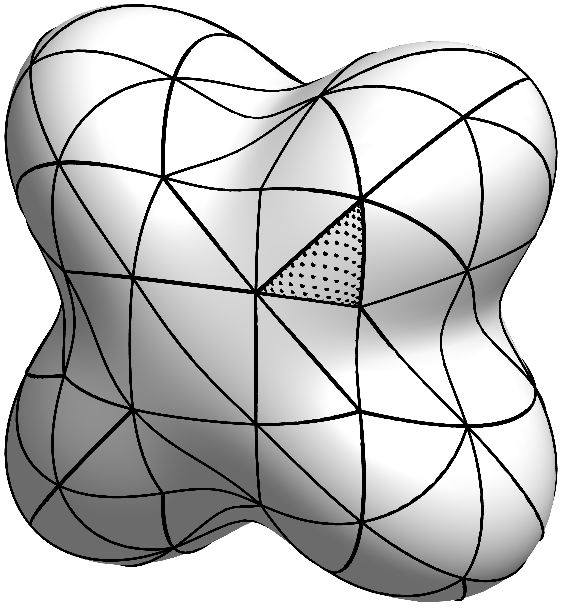
\includegraphics[width=\textwidth,height=0.44\textheight,keepaspectratio]{cushion_geo3.pdf}
\par\footnotesize Triangulated cushion-shaped boundary.
\end{column}
\begin{column}{0.47\textwidth}
\centering
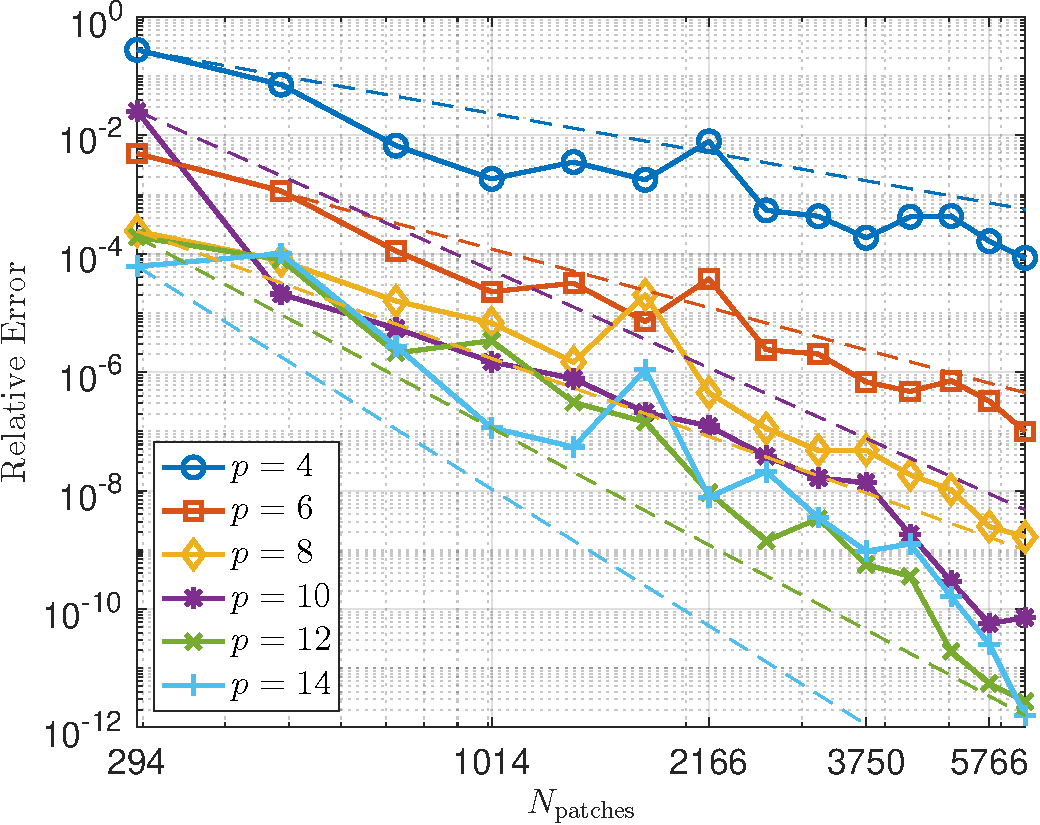
\includegraphics[width=\textwidth,height=0.50\textheight,keepaspectratio]{cushion_convergence.pdf}
\par\footnotesize Relative $\ell_\infty$ error versus $N_{\rm patches}$.
\end{column}
\end{columns}
\vspace{0.5mm}
\begin{block}{Interpretation}
The cubed-sphere construction gives $N_{\rm patches}=12n_\theta n_\phi$; dashed
lines show expected convergence rates. Fine details can be under-resolved by the nonadaptive mesh.
\end{block}
\end{frame}

% 101
\begin{frame}{Stellarator solve at $p=8$: SLP RRQ throughput is close to FMM}
\small
\begin{columns}[T,totalwidth=\textwidth]
\begin{column}{0.52\textwidth}
\centering
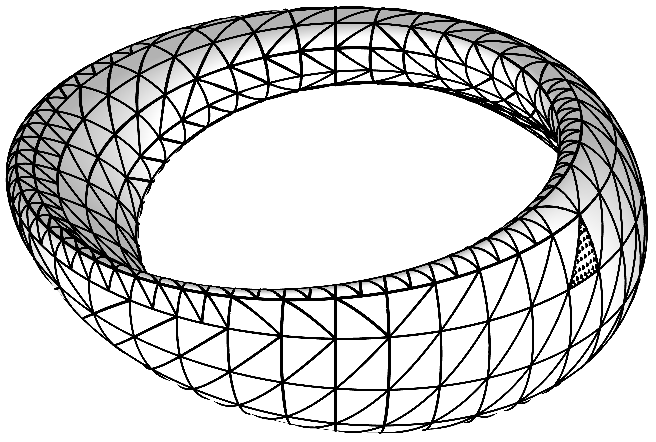
\includegraphics[width=\textwidth,height=0.44\textheight,keepaspectratio]{stellarator_geo.pdf}
\par\footnotesize Triangulated stellarator boundary.
\end{column}
\begin{column}{0.44\textwidth}
\centering
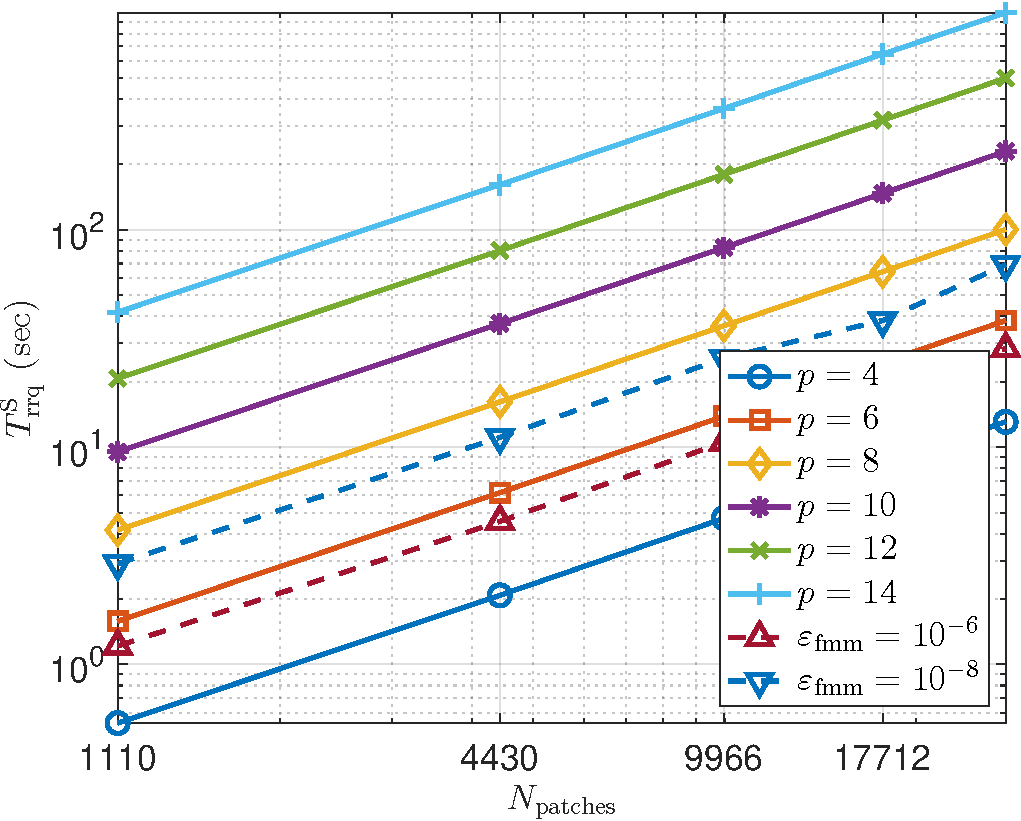
\includegraphics[width=\textwidth,height=0.50\textheight,keepaspectratio]{stellarator_Sinit_SLP.pdf}
\par\footnotesize Single-layer correction time $T_{\rm RRQ}^{S}$.
\end{column}
\end{columns}

\vspace{0.5mm}
\begin{block}{Measured performance}
The plot is the time to build the sparse RRQ correction on the boundary. At $p=8$
($E_\infty=2.76\times10^{-7}$), the SLP RRQ throughput is $9{,}921$ points s$^{-1}$
per core, versus $13{,}983$ for the smooth FMM part. Dashed curves are one FMM call.
\end{block}
\end{frame}

% 102
\begin{frame}{Stellarator solve at $p=8$: DLP RRQ throughput is close to FMM}
\small
\begin{columns}[T,totalwidth=\textwidth]
\begin{column}{0.52\textwidth}
\centering
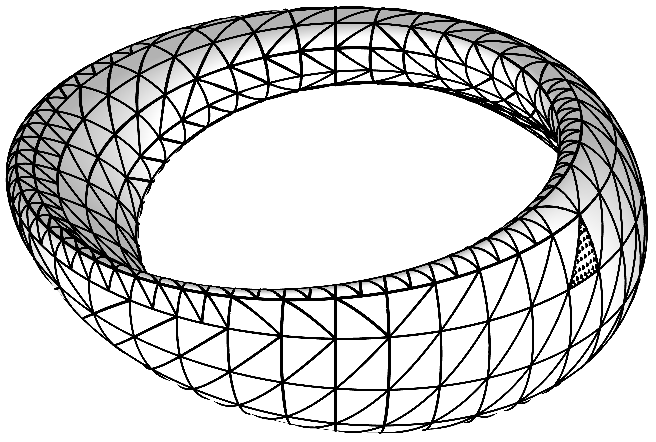
\includegraphics[width=\textwidth,height=0.44\textheight,keepaspectratio]{stellarator_geo.pdf}
\par\footnotesize Triangulated stellarator boundary.
\end{column}
\begin{column}{0.44\textwidth}
\centering
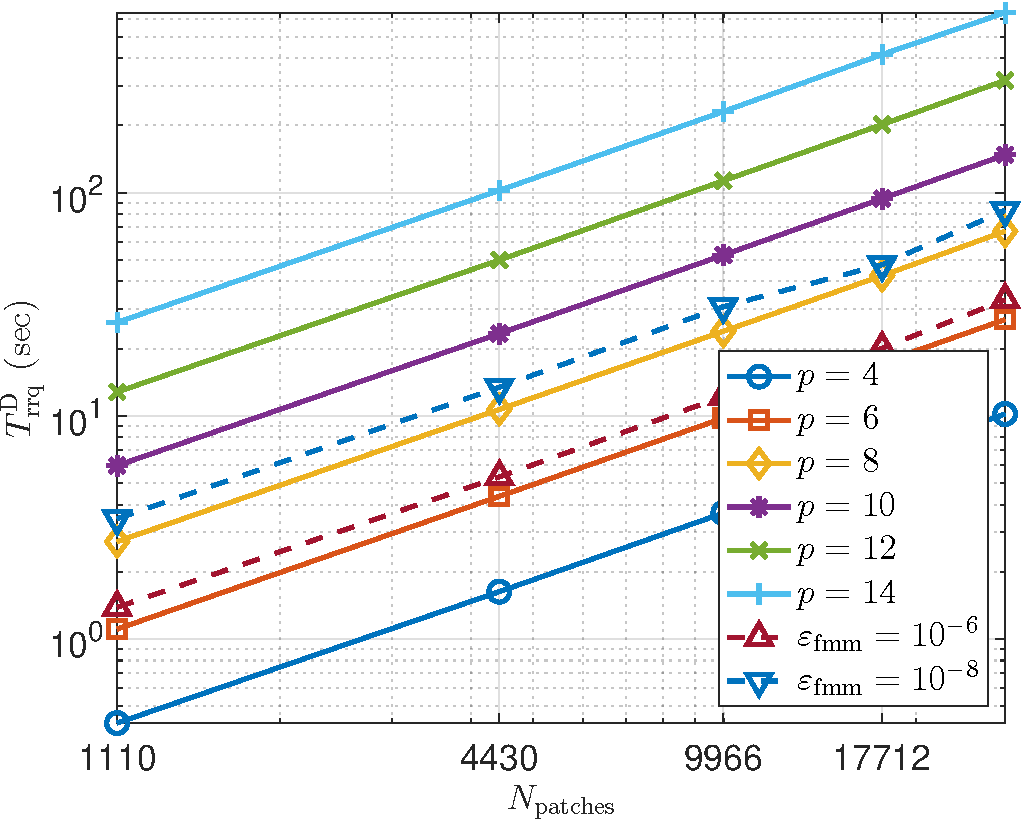
\includegraphics[width=\textwidth,height=0.50\textheight,keepaspectratio]{stellarator_Sinit_DLP.pdf}
\par\footnotesize Double-layer correction time $T_{\rm RRQ}^{D}$.
\end{column}
\end{columns}
\vspace{0.5mm}
\begin{block}{Measured performance}
The plot is the time to build the sparse RRQ correction on the boundary. At $p=8$
($E_\infty=2.76\times10^{-7}$), the DLP RRQ throughput is $15{,}017$ points s$^{-1}$
per core, versus $11{,}646$ for the smooth FMM part. Dashed curves are one FMM call.
\end{block}
\end{frame}

% 103
\begin{frame}{Volume evaluation: throughput is the appropriate RRQ--FMM metric}
\small
\begin{columns}[T,totalwidth=\textwidth]
\begin{column}{0.44\textwidth}
\centering
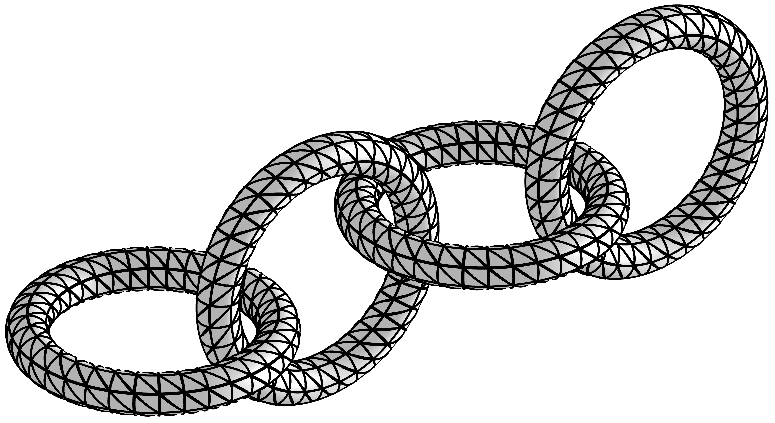
\includegraphics[width=\textwidth,height=0.42\textheight,keepaspectratio]{iltori_geo.pdf}
\par\footnotesize Interlocked-tori geometry.
\end{column}
\begin{column}{0.52\textwidth}
\begin{block}{The two parts process different target sets}
The FMM evaluates the smooth potential at all $N_T$ volume targets. RRQ is used
only for the $N_T^c$ close targets that require special quadrature.
\end{block}
\begin{block}{Throughput normalizes this difference}
\[
  X_{\rm RRQ}^{S}=\frac{N_T^c}{T_{\rm RRQ}^{S}},\qquad
  X_{\rm FMM}^{S}=\frac{N_T}{T_{\rm FMM}^{S}},
\]
with the analogous definitions for the DLP. Absolute correction and FMM times
are therefore not the appropriate performance comparison.
\end{block}
\end{column}
\end{columns}
\end{frame}

% 104
\begin{frame}{Interlocked-tori volume evaluation: RRQ and FMM throughput}
\small
\begin{block}{Result}
At $p=6$ and $p=8$, the RRQ and FMM throughputs are comparable for both layer
potentials.
\end{block}
\vspace{2mm}
\centering
\renewcommand{\arraystretch}{1.22}
\begin{tabular}{c|rr|rr|cc}
  & \multicolumn{2}{c|}{SLP throughput} & \multicolumn{2}{c|}{DLP throughput} & & \\
  $p$ & $X_{\rm RRQ}^{S}$ & $X_{\rm FMM}^{S}$ & $X_{\rm RRQ}^{D}$ & $X_{\rm FMM}^{D}$ & $\varepsilon_{\rm FMM}$ & $E_\infty$ \\
  \hline
  4  & 583{,}929 & 468{,}224 & 687{,}077 & 433{,}446 & $1.00\mathrm{e}{-04}$ & $1.14\mathrm{e}{-04}$ \\
  6  & 272{,}680 & 260{,}129 & 318{,}736 & 250{,}650 & $1.00\mathrm{e}{-06}$ & $1.41\mathrm{e}{-06}$ \\
  8  & 126{,}596 & 140{,}465 & 143{,}307 & 130{,}197 & $1.00\mathrm{e}{-08}$ & $3.22\mathrm{e}{-08}$ \\
  10 & 58{,}368  & 108{,}913 & 65{,}770  & 102{,}488 & $1.00\mathrm{e}{-09}$ & $7.47\mathrm{e}{-10}$ \\
  12 & 28{,}941  & 74{,}238  & 32{,}493  & 69{,}085  & $1.00\mathrm{e}{-10}$ & $1.33\mathrm{e}{-11}$ \\
  14 & 14{,}995  & 55{,}063  & 16{,}584  & 50{,}249  & $1.00\mathrm{e}{-12}$ & $6.11\mathrm{e}{-12}$ \\
\end{tabular}
\par\vspace{1mm}
\footnotesize Throughput is in points s$^{-1}$ per core.
\end{frame}

% 105
\begin{frame}{Comparison with adaptive quadrature}
\small
Adaptive quadrature resolves near singularities by subdividing integration
regions until the kernel is smooth enough.

RRQ reformulates the problem:
\[
  \text{near singularity}
  \quad\longrightarrow\quad
  \text{analytic one-dimensional moments}.
\]

\begin{itemize}
  \item The reported implementation avoids adaptive surface integration for
  classified self, near, and close interactions.
  \item Self, near, and close interactions use one correction construction.
  \item Sparse correction matrices are compatible with FMM-accelerated smooth parts.
\end{itemize}
\end{frame}

% 103
\begin{frame}{Using RRQ inside a BIE solver}
\small
For each matrix-vector product:
\[
  \bm D\mu
  =
  \bm D_{\rm smooth}\mu
  +
  \bm D_{\rm RRQ}\mu.
\]

\begin{itemize}
  \item Apply $\bm D_{\rm smooth}$ using FMM and source quadrature weights.
  \item Apply $\bm D_{\rm RRQ}$ as a sparse correction.
  \item Build or update the sparse correction only when geometry or discretization
  changes.
\end{itemize}
\end{frame}

\begin{frame}{References}
\small
\begin{itemize}
  \item F. Fryklund, L. Greengard, S. Jiang, and S. Potter,
  ``A lightweight, geometrically flexible fast algorithm for the evaluation of
  layer and volume potentials,'' \emph{Journal of Computational Physics},
  547 (2026), 114505.
  \item F. Vico, L. Greengard, and M. Ferrando,
  ``Fast convolution with free-space Green's functions,''
  \emph{Journal of Computational Physics}, 323 (2016), 191--203.
  \item S. Jiang and H. Zhu, ``Recursive reduction quadrature for the evaluation
  of Laplace layer potentials in three dimensions,'' arXiv:2411.08342 (2024).
  \item L. af Klinteberg and A. H. Barnett, ``Accurate quadrature of nearly
  singular line integrals in two and three dimensions by singularity swapping,''
  \emph{BIT Numerical Mathematics}, 61 (2021), 83--118.
\end{itemize}
\end{frame}

\end{document}
